\chapter{Tool demonstration for load-following and safety analysis: 
Transatomic Power MSR}
In order to be competitive in the current domestic energy market, \glspl{MSR} 
may need the flexibility to follow net load on the grid. Such load-following 
operation has the potential to increase the commercial competitiveness of 
nuclear power dramatically. Due to the increasing penetration of renewables 
into the electric grid, base-load operation carries the risk of 
correspondingly frequent negative electric energy pricing. Thus, 
responsiveness to net electricity demand is essential to market relevance 
for new designs \cite{energy_information_administration_u.s._2016}.
This chapter presents a validation demonstration applying SaltProc v1.0 to 
simulate fuel salt depletion with online reprocessing during short-term 
transient to evaluate load-following capabilities of the \gls{TAP} \gls{MSR}.

\section{Technical aspects of load following with nuclear 
reactors}\label{ch5:aspects}

The physical constrains limiting power variations in conventional \glspl{LWR} 
include \cite{lokhov_technical_2011}:
\begin{itemize}[noitemsep, topsep=0pt]
	\item thermal strain and stress to fuel materials\footnote{This constrain 
		does not apply to circulating-fuel \glspl{MSR} because the fuel is 
		into a
		liquid form.};
	\item fuel burnup (low excess reactivity at the \gls{EOC});
	\item \emph{$^{135}$Xe poisoning (iodine pit)};
	\item reactivity thermal feedback (change in the temperature of the 
	primary coolant and fuel causes negative reactivity insertion which limits 
	power regulation capabilities).
\end{itemize}
Each of these physical effects is currently under active international 
research. 

This chapter focuses only on the fission product poisoning, especially the 
``iodine pit''. The ``iodine pit'', also called the ``iodine hole'' or ``xenon 
pit'', is the reactor's inability to start a few hours after the reactor power 
decreases due to peak of $^{135}$Xe concentration in the core.
The $^{135}$Xe is the strongest known neutron absorber 
($\sigma_{a,^{135}Xe}=2.6\times10^6$ barns) with a half-life 
$\tau_{1/2}=9.17h$ and yield for $^{235}$U fission about 6.6\%. 
Figure~\ref{fig:xe-reaction-chain} shows the entire decay chain, which 
characterizes $^{135}$Xe gain and loss channels. The vast 
majority of $^{135}$Xe (6.4\%) is produced from $^{135}$I decay 
($\tau_{1/2}=6.6h$). About half of $^{135}$I is produced directly from fission 
and half from $^{135}$Te decay ($\tau_{1/2}=19s$) 
\cite{nuclear_power_production_2020}.
\begin{figure}[hbp!] % replace 't' with 'b' to 
	\centering
	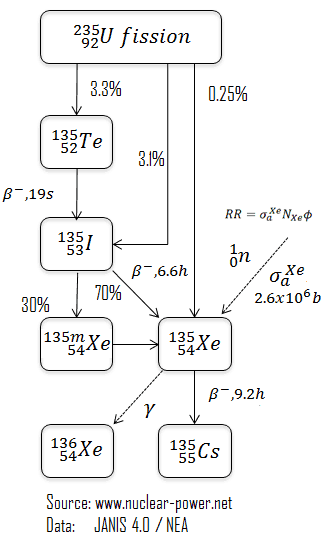
\includegraphics[width=0.4\textwidth]{ch5/xenon-135-reactions-decay.png}
	\caption{Mechanisms of $^{135}$Xe gain and loss in the reactor core 
		(reproduced from \cite{nuclear_power_production_2020}).}
	\label{fig:xe-reaction-chain}
\end{figure}

Under normal operating conditions, $^{135}$Xe is transmuted to $^{136}$Xe 
(`burned out') in the reactor core as it is produced. 
So, while it harms the neutron economy, balancing the reactor controls can 
compensate for its effect. The burnout of $^{135}$Xe for an operating reactor 
can be described as follows:
\begin{align}
& \isotope[135]{Xe}+\isotope[1]{n}\rightarrow \isotope[136]{Xe} \;(stable)
\end{align}

Because $^{135}$Xe is produced partially from the $^{135}$I decay, the 
$^{135}$Xe concentration directly depends on the $^{135}$I concentration. 
Therefore, the iodine and xenon rate of change can be described as follows
\begin{align}
\frac{dI(t)}{dt} &= \gamma_I \Sigma_f\phi - \lambda_II \label{eq:iodine}\\
\frac{dX(t)}{dt} &= \lambda_II+\gamma_X\Sigma_f\phi - \lambda_XX - 
\sigma_{a,X}\phi X \label{eq:xenon}
\intertext{where}
I, X &= \mbox{number density of $^{135}$I, $^{135}$Xe [cm$^{-3}$]} 
\nonumber\\
\gamma_I,\gamma_X &= \mbox{effective yield of $^{135}$I, $^{135}$Xe 
	[fission$^{-1}$]} \nonumber\\
\lambda_I,\lambda_X &= \mbox{decay constant of $^{135}$I, $^{135}$Xe 
	[s$^{-1}$]}\nonumber\\
\Sigma_f &= \mbox{macroscopic fission cross section of $^{235}$U [s$^{-1}$]} 
\nonumber\\
\sigma_{a,X} &= \mbox{microscopic absorption cross section of $^{135}$Xe 
	[b]}\nonumber\\
\phi &= \mbox{neutron flux [$cm^{-2}s^{-1}$].}\nonumber
\end{align}

The difficulty comes when the reactor power is reduced, and there are fewer 
neutrons to burn the $^{135}$Xe out, so its concentration increases and 
further suppresses reactor power. In this case, the core takes some time to 
recover from the power reduction impact of $^{135}$Xe. This response to 
changing power levels, particularly from higher to lower power, 
dramatically slows the reactor's response to power demand
\cite{lokhov_load-following_2011}. 

In a liquid-fueled \gls{MSR}, gaseous fission products (e.g., xenon) can be 
dynamically removed from the fuel salt by the gas separation system (see 
Section~\ref{sec:gas-separ}). Thus, xenon gas, including problematic 
$^{135}$Xe, can be removed from the fuel salt outside the reactor core to 
eliminate its negative impact on the core neutronics. If the gas separation 
system can remove the vast majority of xenon, it is possible to alter the 
reactor power output in a wide range with very brief required recovery time. 
Overall, $^{135}$Xe removal during reactor operation would potentially allow 
precise and flexible dynamic control of the reactor power level to follow 
power demands, typically referred to as `load following.'

This chapter presents modeling and simulation of load following transient 
operation of the \gls{TAP} \gls{MSR}. This study focuses on the 
$^{135}$Xe/$^{135}$I balance in the \gls{TAP} core and its effect on 
reactor performance. In this chapter, I simulated short-term ($<24$ hours) 
depletion with the core power changing in the [0,100\%] range for xenon 
removal efficiency ($\epsilon_{Xe}$) varied between 0 and 0.915 (see 
Table~\ref{tab:gas_removal_efficiency}). 

This chapter also demonstrates an analysis of reactor load-following 
capability for various moderator configurations and fuel salt compositions to 
bound the necessary efficiency of the gas removal system to ensure 
load-following operation. 

\section{TAP MSR load following analysis}
All of the analysis herein used SaltProc v1.0 with the full-core 3-D model of 
the \gls{TAP} \gls{MSR} developed using Serpent 2 (see 
Section~\ref{sec:tap_model}). The multi-component, online reprocessing system 
model with realistic noble gas removal efficiency described in 
Section~\ref{sec:tap-online-model}, is used to simulate fission product 
removal and fresh fuel injection during the anticipated transient. To
simulate transients with time-dependent power generation, I added to SaltProc 
v1.0 a new capability to perform fuel salt depletion with variable time 
step size and power level\footnote{For simplicity, the reactor power level 
is adjusted by changing the normalization factor in Serpent (\emph{set power 
P[W]}). This simplification assumes that spatial and energy distribution of 
the neutron flux remains constant and only the magnitude of the flux changes 
with time. That is, control rod movement and the corresponding change in the 
flux spatial and energy distribution are not treated here.} during each 
depletion step. The depletion calculation in the load following regime 
captures the effects of $^{135}$Xe poisoning and illuminates the benefit of 
using an online gas removal system in the \gls{TAP} concept.

\subsection{Power load curve selection approach}\label{sec:worst-load}
The load and generation must be continuously and almost instantly balanced in 
an electric power system. This is a physical requirement independent of the 
market structure. Regulation and load following (in the real-time energy 
market they are provided  by the 
intra-hour workings) are the two services 
required to maintain a balance between power generation and power load. 
Figure~\ref{fig:power-curve-ny} demonstrates the morning ramp-up decomposed 
into the total load (green), smooth load-following ramp (blue), and regulation 
(red). The smooth load-following slowly rises from 3566 MW to 4035 MW over 3 
hours. Regulation compensates for high-frequency fluctuations in the load 
around the underlying trend within the $\pm55$MW range. In the PJM region 
(Delaware, Illinois, Indiana, Kentucky, Maryland, Michigan, New Jersey, North 
Carolina, Ohio, Pennsylvania, Tennessee, Virginia, West Virginia, and the 
District of Columbia), New York, and New England, the 5-min ramping capability 
of a generator is required for the regulation, while in Texas and California 
it is 15-min and 10-min, respectively \cite{kirby_method_2005}.
\begin{figure}[htp!] % replace 't' with 'b' to 
	\centering
	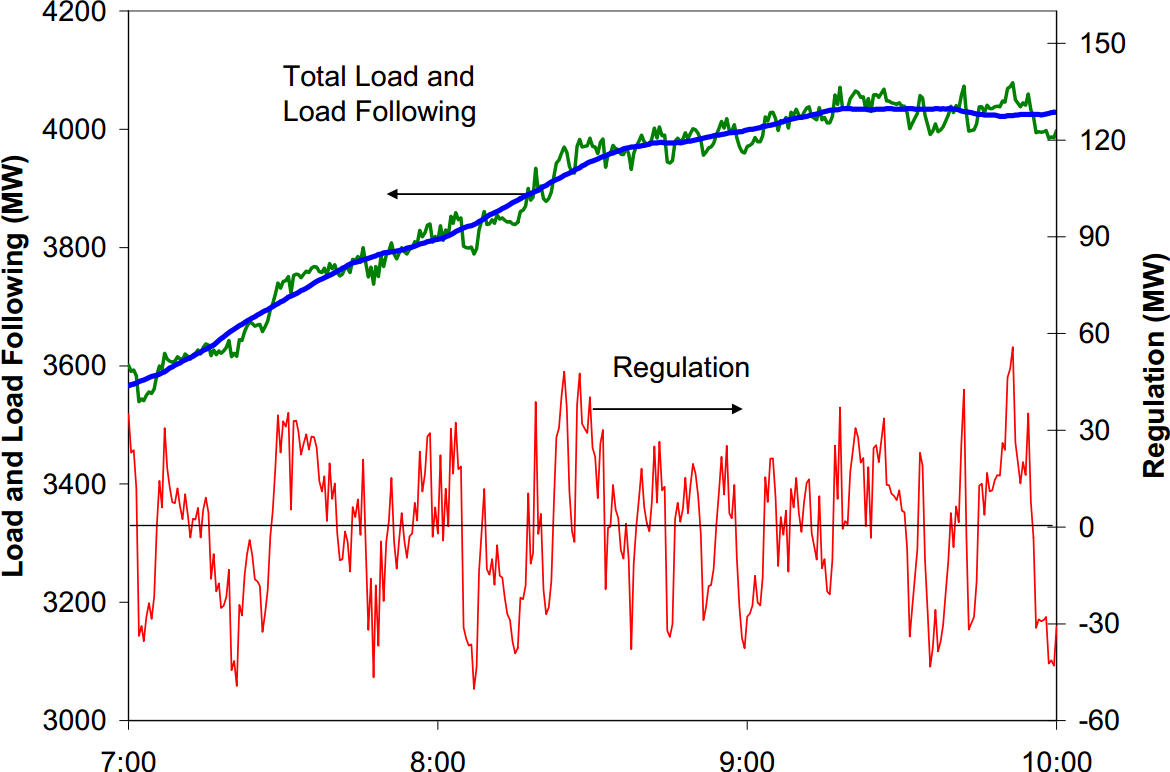
\includegraphics[width=0.85\textwidth]{ch5/power-curve-ny-morning.png}
	\caption{Regulation (red) compensates for minute-to-minute fluctuations in 
	system total load (green), load following (blue) compensates for the 
	inter- and intra-hour ramps (reproduced from \cite{kirby_method_2005}).}
	\label{fig:power-curve-ny}
\end{figure}

In this context \emph{regulation} refers to the use of online generation or 
storage that is equipped with automatic generation control and can change 
output quickly (MW/min ramp rate) to compensate for the minute-to-minute 
fluctuations in customer loads and correct for unintentional fluctuations
in power generation \cite{kirby_method_2005}. Typical natural gas peaking 
plants can ramp at or above 10\% of their capacity per minute 
\cite{huff_enabling_2018}. Elite combustion engine peakers (W\"{a}rtsil\"{a}) 
can ramp up from 10\% to 100\% load (or down) in less than one minute 
\cite{wartsila_combustion_2020}. Hydropower plants also typically have 
accurate, high-speed ramping capability suitable for regulation 
\cite{kirby_method_2005}.

Conventional nuclear power plants (Generation III/III+) can be used for 
load-following (blue curve on Figure~\ref{fig:power-curve-ny}) but have 
limited maneuverability. For example, the German Konvoi reactors 
are designed for 15,000 cycles with daily power variations from 100\% to 60\% 
power level with ramp rate up to 2\%/min \cite{ludwig_load_2011}, which is by 
order of magnitude slower than fossil-fueled plants. 
The \glspl{MSR} must enable daily power variation with a much more flexible 
range (from 100\% to 0\% and from 0\% to 100\%) and ramp rate up to 10\%/min 
to compete with these generators. The physical constrains limiting power 
variation range and ramp rate in nuclear reactors was listed in 
Section~\ref{ch5:aspects}. 
\emph{The current chapter of the dissertation focuses only on the $^{135}$Xe 
poisoning effect.} Other physical effects, such as thermal strain and stress 
in structural materials are not treated here.


Performing a depletion calculation with SaltProc v1.0 to mimic the 
load-following maneuvering shown in Figure~\ref{fig:power-curve-ny} would 
require a very fine time step (e.g., 15-minute step). To simulate power change 
with the desired rump rate (0.1 \gls{HFP}/min), depletion time step resolution 
of less than a 1-minute is needed. 
Such fine resolution requires thousands of depletion time steps to simulate 
12-hour transient involving unreasonable computational costs. 
Instead, this chapter presents simulations with a 1-hour time step to 
investigate the impact of gaseous fission product removal on the reactor 
response to power demands. 

The most challenging power transient for conventional \glspl{LWR} from the 
viewpoint of xenon poisoning is well-defined in the literature. If after the 
$^{135}$Xe concentration reaches equilibrium (40-50 hours after startup with 
fresh fuel), the reactor power was decreased from 100\% to 0\% (e.g., the 
reactor is tripped), the $^{135}$Xe concentration and corresponding negative 
reactivity insertion would reach maximum in about 10-11 hours after shutdown 
\cite{lamarsh_introduction_1975, 
bell_nuclear_1970}. Notably, the time after 
shutdown when $^{135}$Xe concentration reaches a maximum strongly depends on 
the reactor neutron energy spectrum.

Thus, to demonstrate SaltProc v1.0 capabilities for a short-term transient 
with 
the reactor power change and to investigate load-following capabilities of the 
\gls{TAP} reactor with a focus on the xenon poisoning, I selected following 
worst-case power load profile:
\begin{enumerate}[label=(\alph*), noitemsep, topsep=0pt]
	\item operate on 100\% of \gls{HFP} long enough to reach 
	$^{135}$I/$^{135}$Xe equilibrium;
	\item instantaneous power drop from 100\% to 0\%;
	\item shutdown for $t^{max}_X$ [hours] to reach the $^{135}$Xe 
	concentration extremum;
	\item restart the reactor instantly from 0\% to 100\% power level and 
	operate on 100\% for a few hours.
\end{enumerate}
Or in math formulation:
\begin{align}
P(t)& = 
\begin{cases}
100\%,&  t < t_{eq}\\
0\%,  &  t_{eq} \leq t \leq t_{eq}+t^{max}_X\\
100\%,&  t > t_{eq}+t^{max}_X
\end{cases}
\intertext{where}
P(t) &= \mbox{reactor power level [\%]} \nonumber\\
t_{eq} &= \mbox{time after startup to reach $^{135}$Xe equilibrium 
concentration [h]} 
\nonumber\\
t^{max}_X &= \mbox{time after shutdown when $^{135}$Xe concentration peaks 
[h].}\nonumber
\end{align}
This postulated worst-case transient could be considered as backing up solar 
power with nuclear on a high-solar-penetration grid (e.g., in California).
Any other power load profile (i.e., blue load-following line shown in  
Figure~\ref{fig:power-curve-ny}) would demonstrate a significantly milder 
xenon poisoning effect because of the power demand change in the [0,100\%] 
range realistically is not instantaneous. That is, if the \gls{TAP} \gls{MSR} 
would be able to maintain criticality in the described stress test (e.g., 
$k_{eff}>1.0$ during all stages of the transient), then it is capable of 
following a realistic load curve.

The local extremum of xenon concentration can be described as follows
\begin{align} \label{eq:xe-extremum}
\frac{dX(t)}{dt} &= 0
\end{align}
The system of Ordinary Differential Equations which consist of 
Equations~\ref{eq:iodine}, \ref{eq:xenon}, and \ref{eq:xe-extremum} must be 
solved to calculate when the $^{135}$Xe concentration reaches maximum.

If the $^{135}$I and $^{135}$Xe concentrations at shutdown is $I_0$ and $X_0$, 
respectively, the time after shutdown when the $^{135}$Xe concentration peaks 
is given by:
\begin{align}\label{eq:time-xe-max}
t^{max}_X &= \frac{1}{\lambda_X-\lambda_I}
log\left(\frac{\lambda_X(\lambda_I[X_0+I_0]-\lambda_XX_0)}{\lambda_I^2 
I_0}\right)
\end{align}

Since the $^{135}$I and $^{135}$Xe concentrations at shutdown in the \gls{TAP} 
core are expected to be different at the \gls{BOL} and \gls{EOL} due to 
significant spectral shift, $t^{max}_X$ is recalculated for each case to 
obtain the worst possible xenon poisoning effect. The ultimate goal of this 
effort is to evaluate the timing and impact of problematic fission product 
removal (i.e. xenon removal) on maximum negative reactivity insertion.



\subsection{Results and Analysis}
The \gls{TAP} full core depletion analysis was performed using SaltProc v1.0. 
A 1-hour depletion time step captures rapid changes in reactivity and 
isotopic composition during the transient. 
Figure~\ref{fig:lf-tap-keff-eol-eoc-no} demonstrated the effective 
multiplication factor evolution during postulated worst-case transient when 
the reactor is tripped for $11$ hours (typical time to reach maximum 
$^{135}$Xe concentration in conventional \glspl{LWR}) and then restarted. 
\emph{The gas removal system for that demonstration case was inactive to 
enhance the xenon poisoning effect.} At the beginning of the transient 
(initial conditions), the reactor operated for 8448 days ($\approx23$ years), 
and all moderator rods are inserted in the core (see 1668 rods configuration 
in Figure~\ref{fig:tap-840-1668}). The negative effect of xenon poisoning is 
expected to be the greatest at the \gls{EOL} when the core has the most 
thermal neutron spectrum. 
The multiplication factor decreases by 64 $pcm$ during the first two hours 
after shutdown ($^{135}$Xe concentration reached its maximum) and then 
increases by 242 $pcm$ because $^{135}$Xe loss due to decay overcame its gain 
from $^{135}$I decay. The $k_{eff}$ increase accelerated after reactor power 
turned back to 100\% due to $^{135}$Xe burnout. 
Figure~\ref{fig:lf-tap-keff-eol-eoc-no} clearly indicates that the time after 
shutdown when the $^{135}$Xe reaches its extremum ($t^{max}_X$) is 
significantly shorter for the \gls{TAP} reactor than for \glspl{LWR} (11 
hours).
\begin{figure}[htp!] % replace 't' with 'b' to 
	\centering
	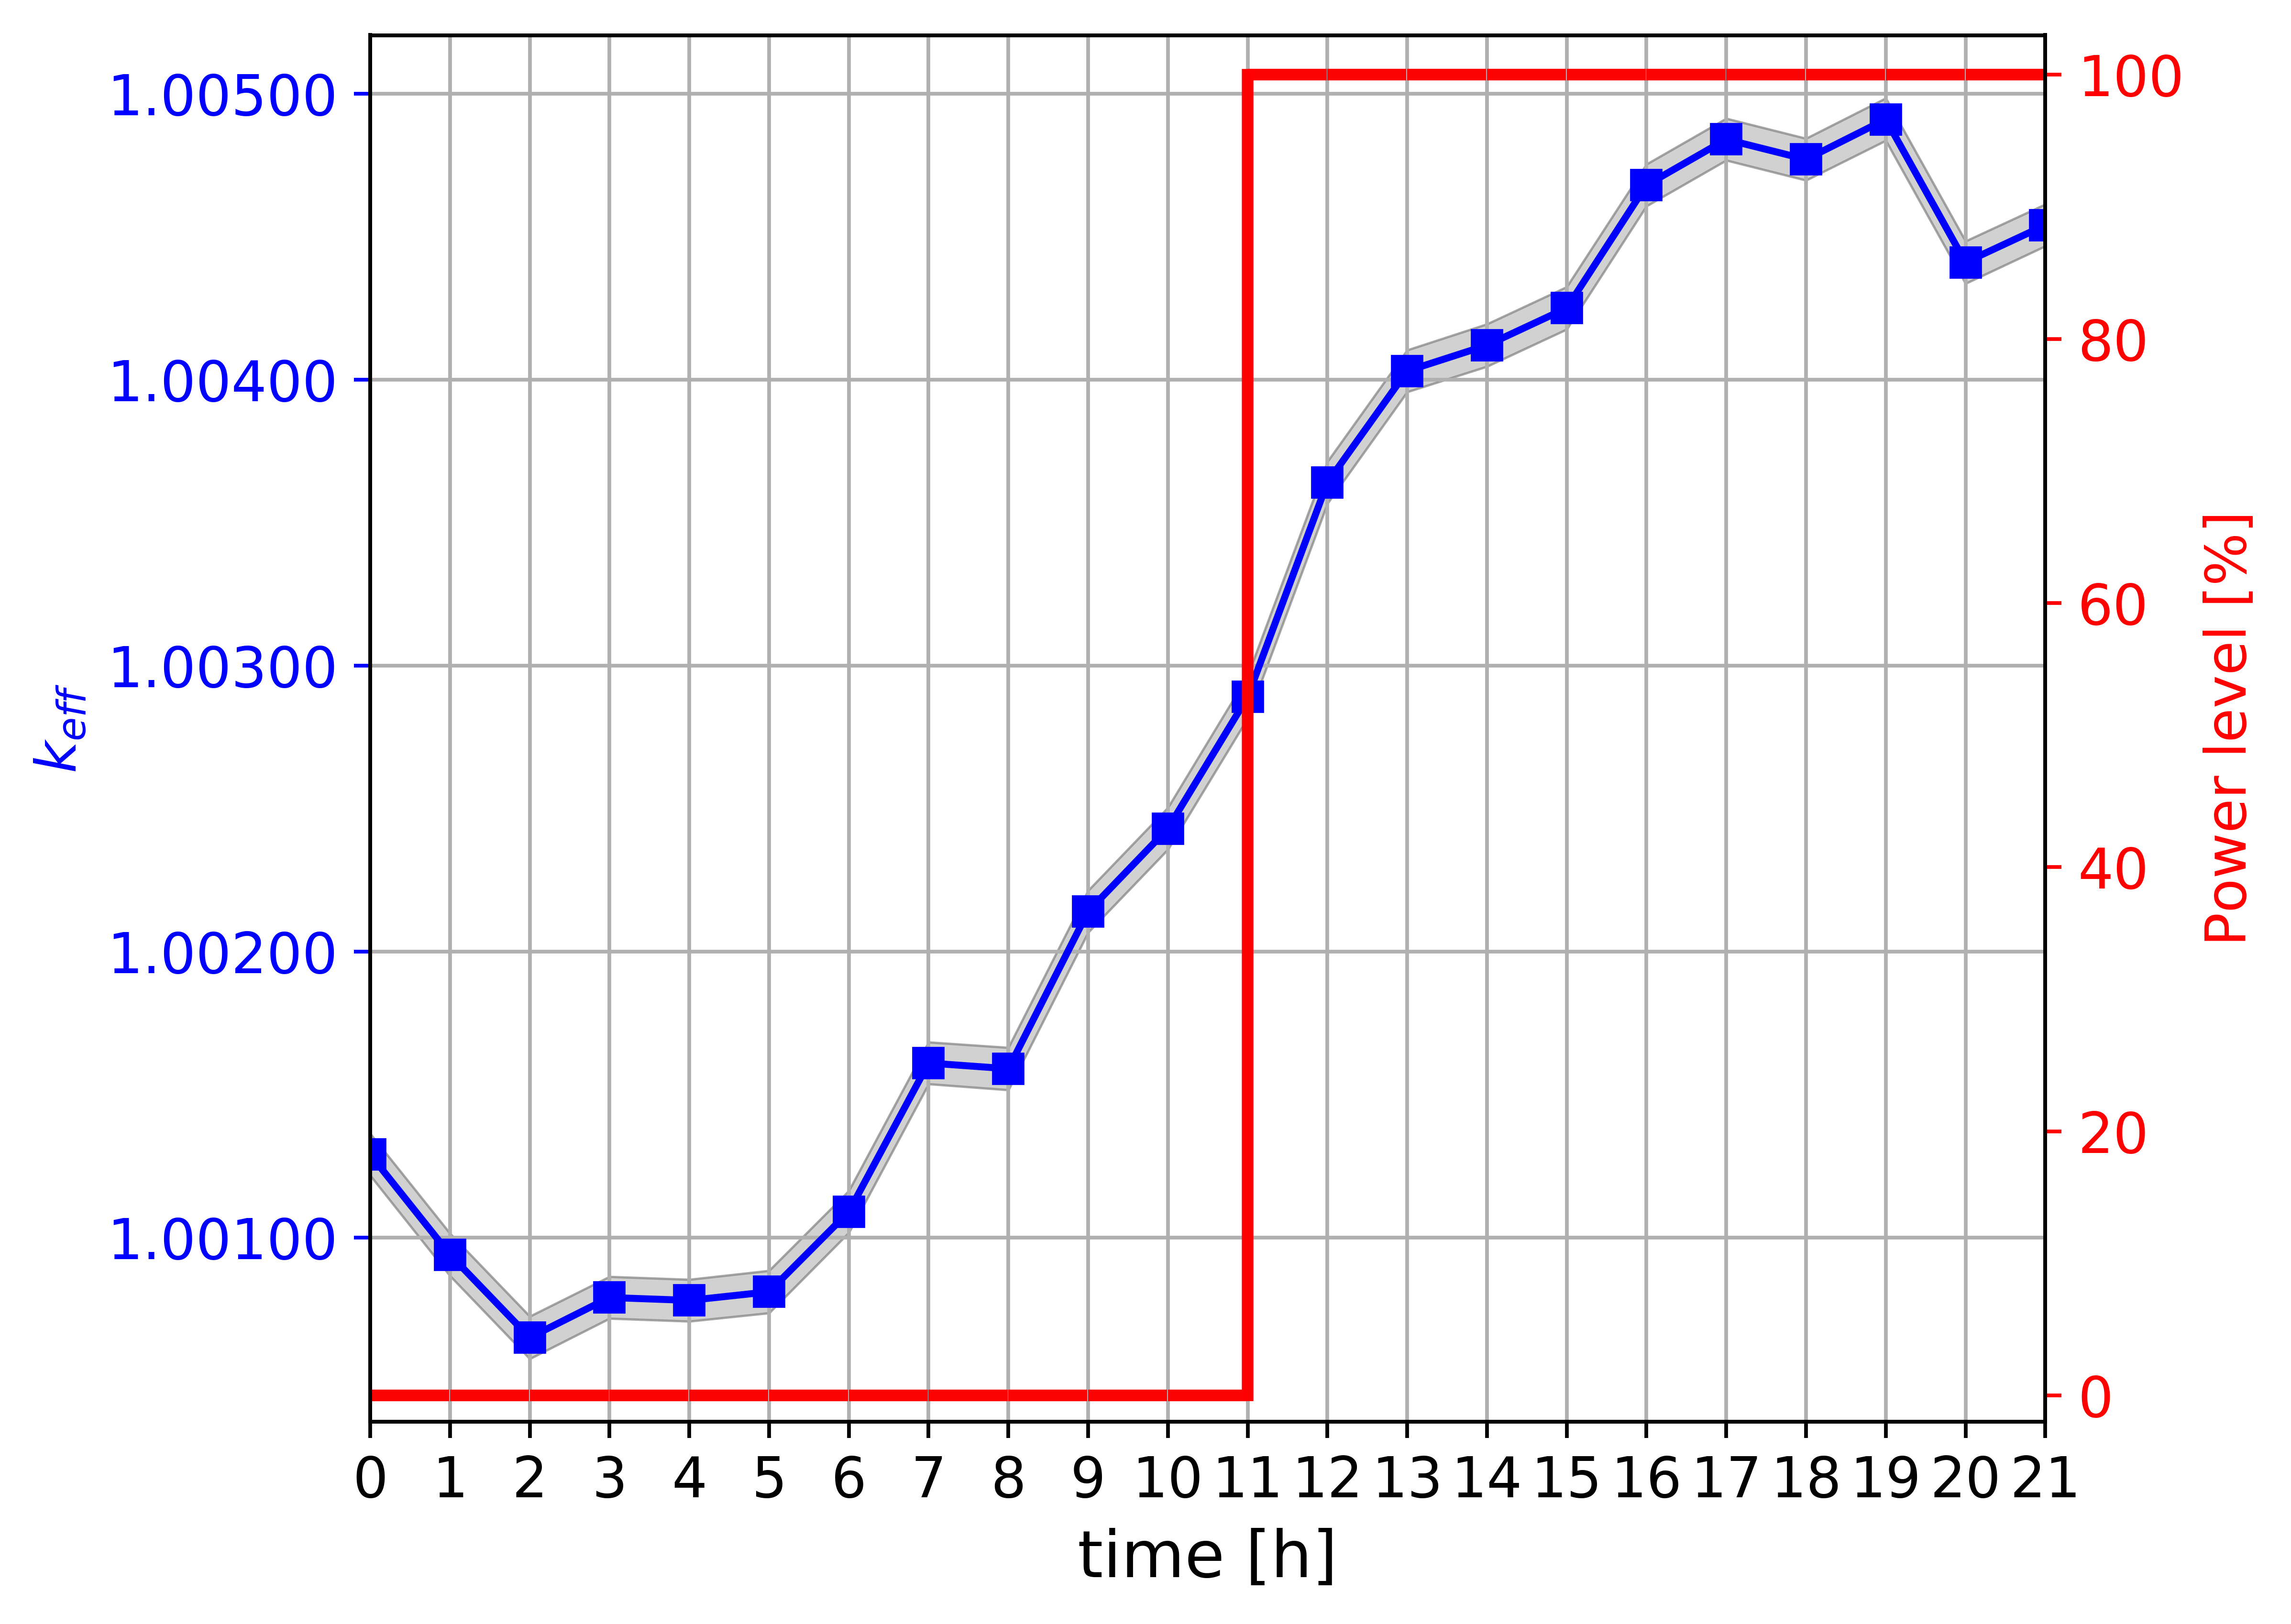
\includegraphics[width=0.9\textwidth]{ch5/keff_kl_1_eol_eoc.png}
	\caption{The effective multiplication factor dynamics for an 11-hour 
		shutdown (well-known xenon peak time for \glspl{LWR}) for the TAP 
		reactor, 
		10 days before the \gls{EOL} (all moderator rods inserted), the gas 
		removal system is turned off. Uncertainty ($\sigma\pm7$ $pcm$) is 
		shaded.}
	\label{fig:lf-tap-keff-eol-eoc-no}
\end{figure}

Using $^{135}$I and $^{135}$Xe number densities at the 8448$^{th}$ day of 
operation (the 10$^{th}$ day before the \gls{EOL}) from long-term realistic 
analysis 
(see Section~\ref{sec:long-term-real}) and Equation~\ref{eq:time-xe-max}, I 
calculated the xenon peak time for the \gls{TAP} \gls{MSR} with all moderator 
rods inserted: $t^{max}_X=2.76h$. To estimate maximum negative reactivity 
insertion due to xenon poisoning, the transient simulation is repeated with 
the finer time resolution (15 minutes instead of 1 hour) and shutdown time of 
2.75 hours (e.g., the time between the shutdown and power ramp-up to 100\% is 
equal $t^{max}_X$).

Figure~\ref{fig:lf-tap-keff-eol-eoc-no-15} shows that the effective 
multiplication factor dropped by 70 $pcm$ during the first 2.75 hours after 
shutdown as predicted by Equation~\ref{eq:time-xe-max}. After power ramps up 
from 0\% to 100\%, $k_{eff}$ returned to its initial value (1.00151) in 75 
minutes. The imbalance between $^{135}$I production and $^{135}$Xe burnout is 
the main reason for this positive reactivity boost. Notably, maximum negative 
reactivity insertion due to $^{135}$Xe buildup after shutdown in the 
\gls{PWR} ($-1500$ $pcm$) is two orders of magnitude greater than in the 
\gls{TAP} \gls{MSR} ($-70$ $pcm$).
Thus, the \gls{TAP} reactor with inactive gas removal system remains critical 
throughout worst-case power change even during the 8448$^{th}$ of operation 
(the 10$^{th}$ day before $k_{eff}$ drops below 1) when operative excess 
reactivity is low ($151pcm>70pcm$). If the shutdown happens during the last 9 
days of the \gls{TAP} reactor operation, then the operator would not be able 
to restart it until $t^{max}_X=2.76h$ after shutting down.
\begin{figure}[htp!] % replace 't' with 'b' to 
	\centering
	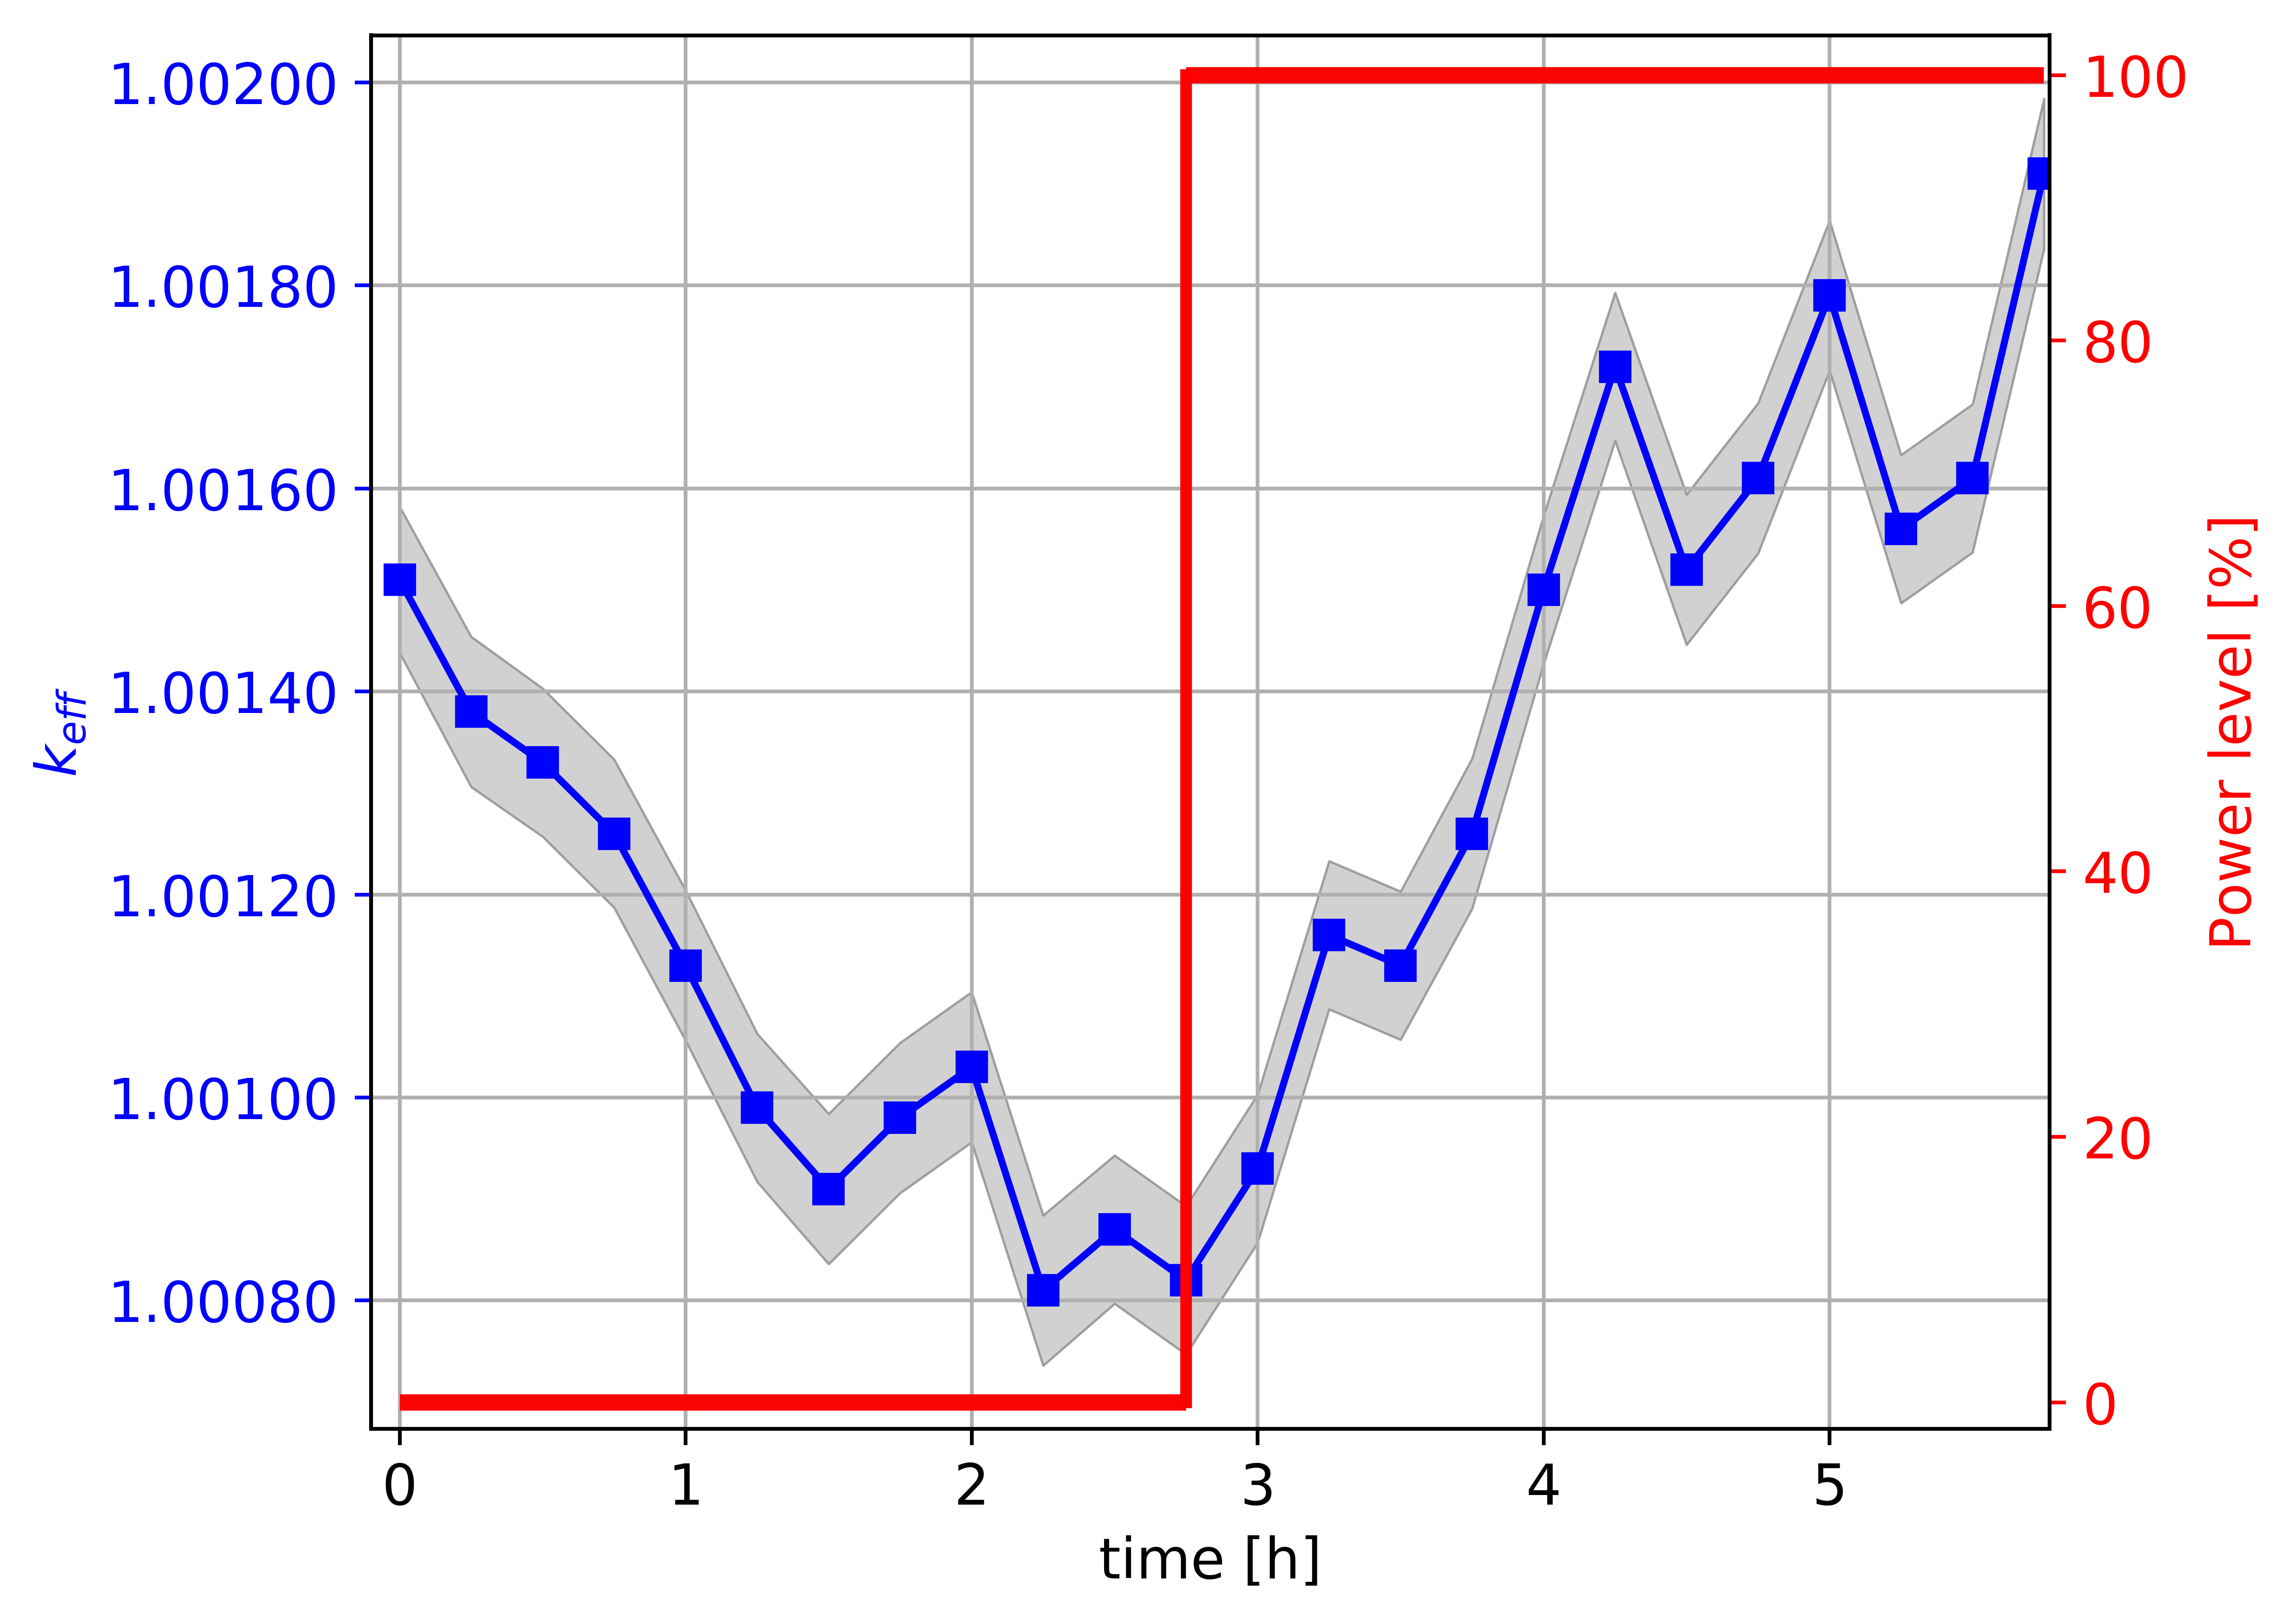
\includegraphics[width=0.9\textwidth]{ch5/keff_kl_1_eol_eoc_15min.png}
	\caption{The effective multiplication factor dynamics for the worst-case 
		load curve (2.75-hour shutdown) for the \gls{TAP} reactor, 10 days 
		before the \gls{EOL} (all moderator rods inserted), the gas removal 
		system is turned off. Uncertainty ($\sigma\pm7$ $pcm$) is shaded.}
	\label{fig:lf-tap-keff-eol-eoc-no-15}
\end{figure}


The analysis of the fuel composition evolution provides clearer information 
about the $^{135}$Xe/$^{135}$I equilibrium and the core state. 
Figure~\ref{fig:lf-tap-xe-i-eol-eoc-no-15} shows changes in the number density 
of isotopes influential to the \gls{TAP} core neutronics throughout the 
transient. The $^{135}$I/$^{135}$Xe number density ratio after reaching xenon
equilibrium is equal to 1.0. After shutdown, $^{135}$I decays to $^{135}$Xe 
that is not burned up. The $^{135}$I decay caused xenon concentration to 
increase by 4\% from equilibrium after 2.75 hours due to a shorter $^{135}$I 
half-life ($\tau_{1/2}(^{135}I)=6.6h$ vs. $\tau_{1/2}(^{135}Xe)=9.17h$). Thus, 
during the first 2.75 hours, $^{135}$Xe gain from $^{135}$I decay slightly 
overcame $^{135}$Xe decay loss. In sum, the $^{135}$Xe peak is almost 
negligible (+4\%) even in the worst-case load profile scenario due to a lower 
$^{135}$I/$^{135}$Xe concentration ratio at the equilibrium: 1.0 and 2.3 for 
the \gls{TAP} reactor and \gls{PWR}, respectively 
\cite{rykhlevskii_impact_2019}.
\begin{figure}[htp!] % replace 't' with 'b' to 
	\centering
	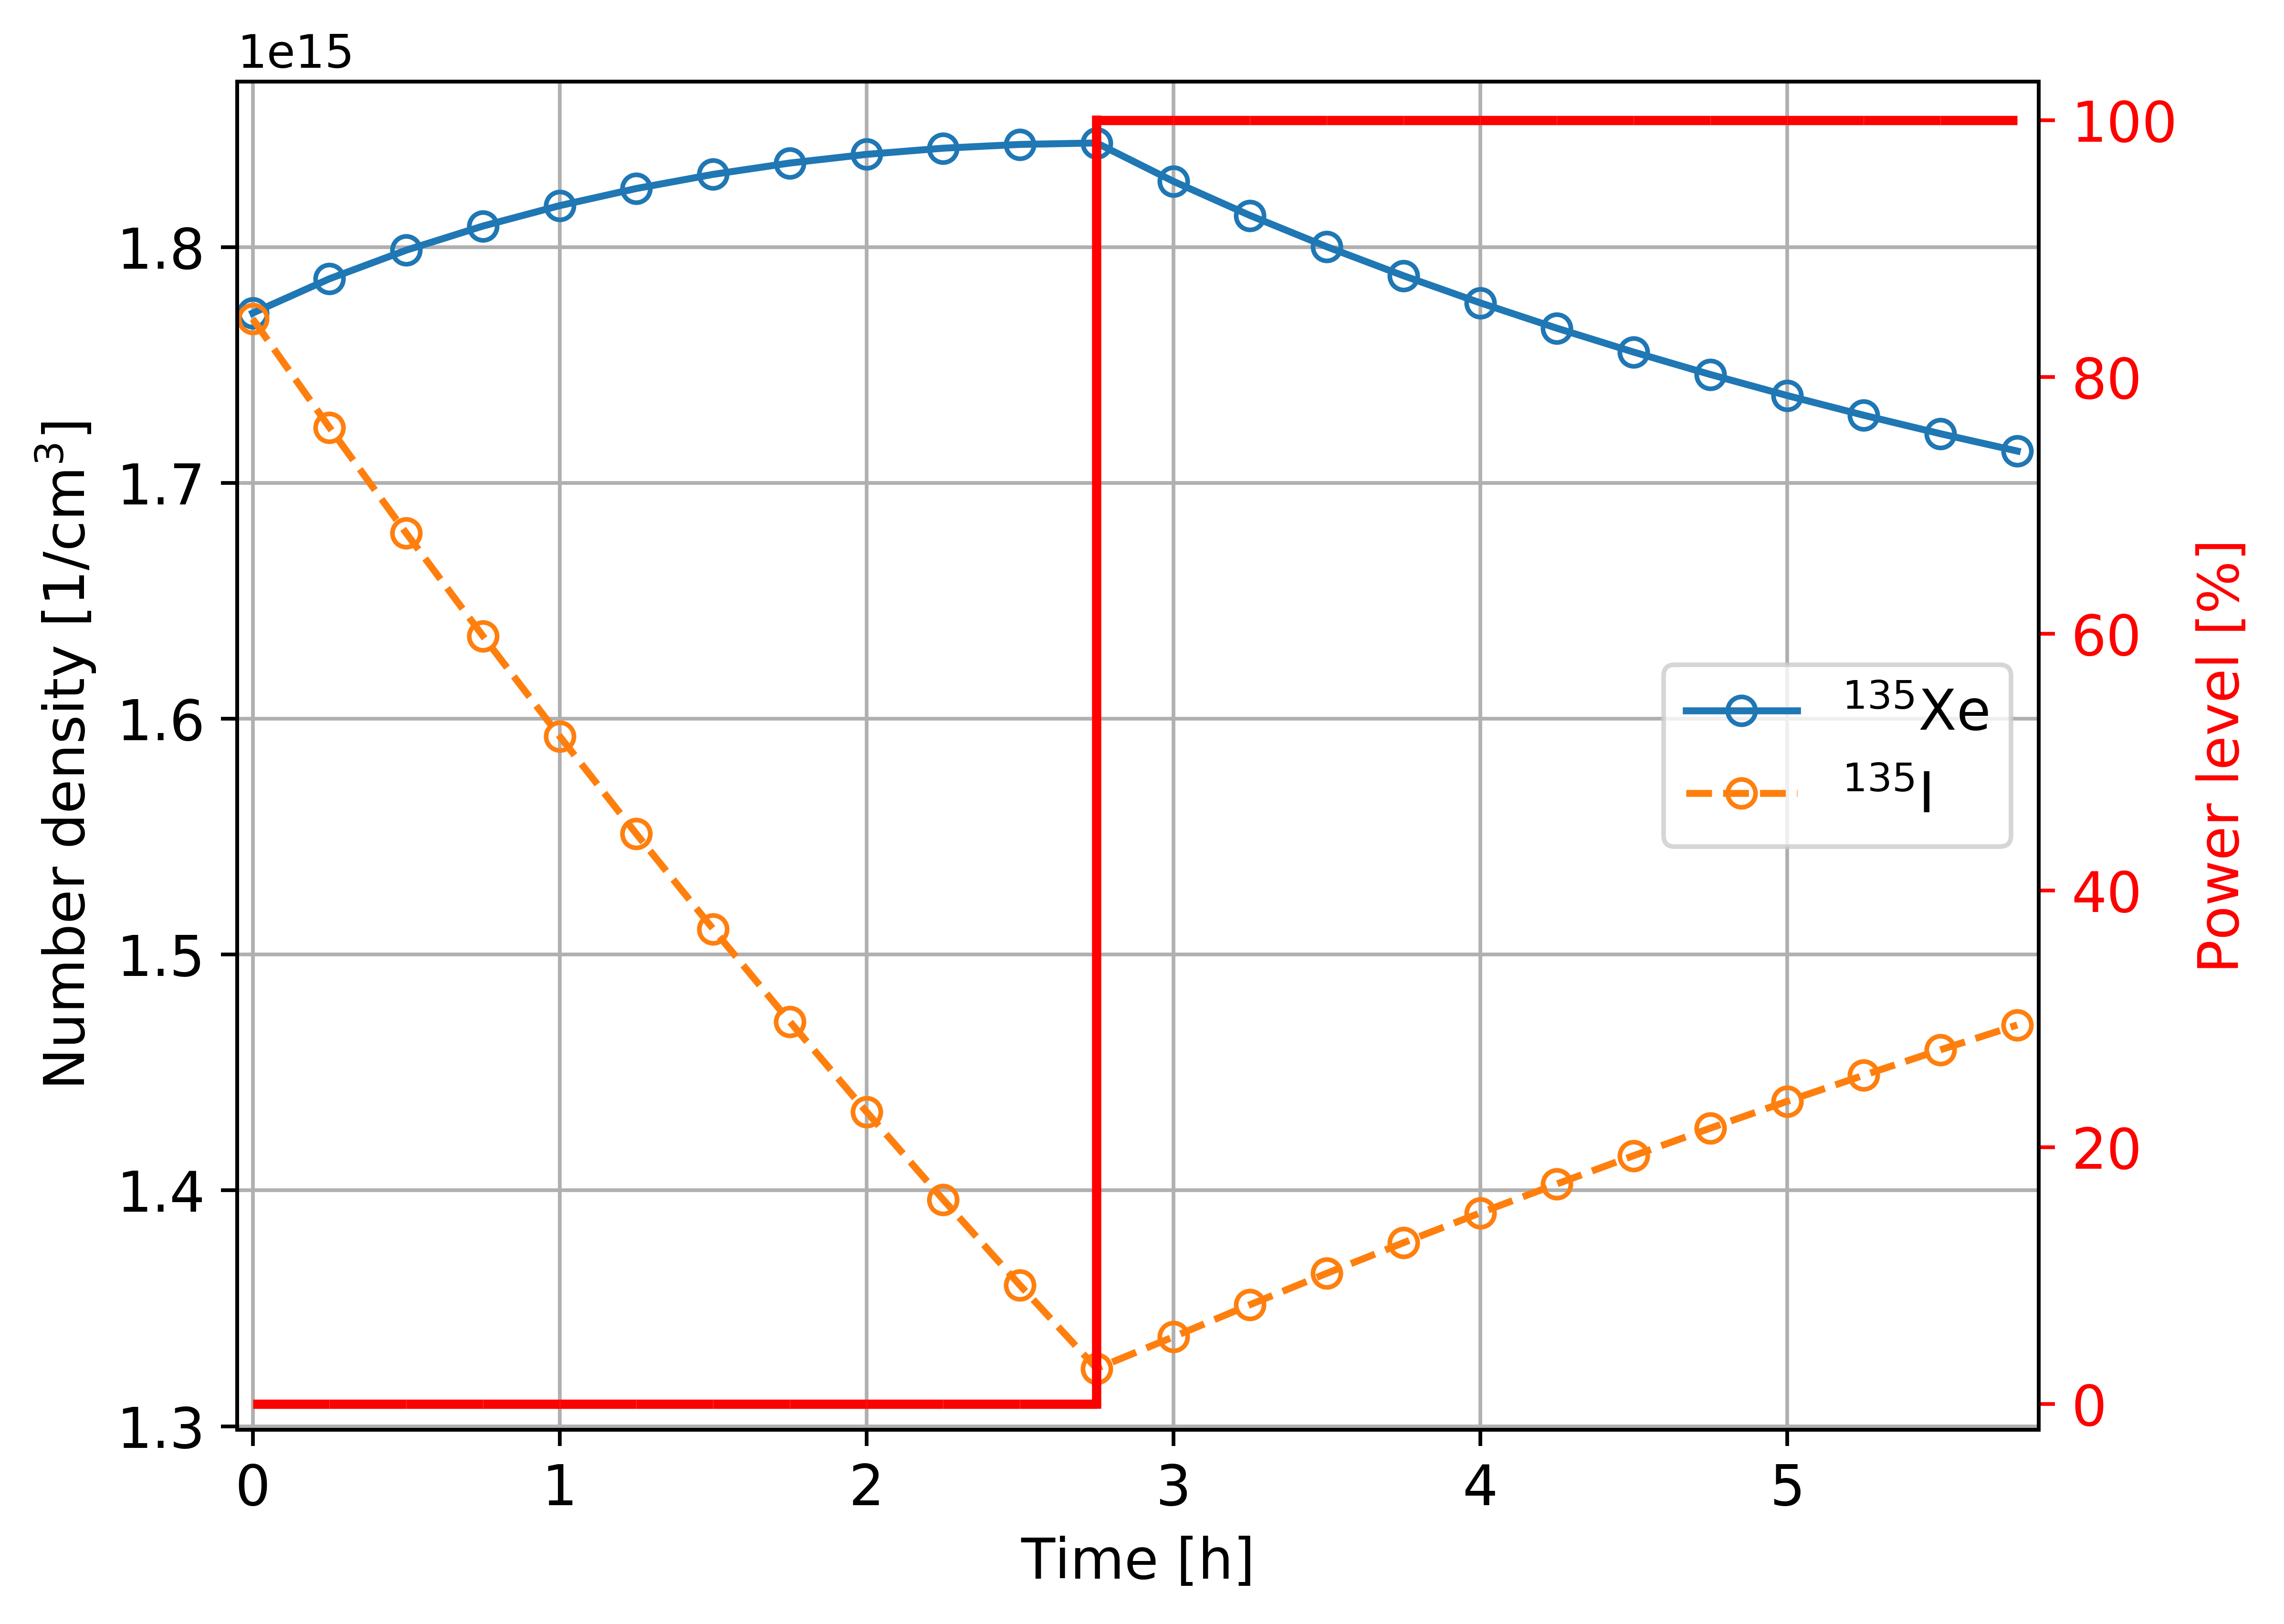
\includegraphics[width=\textwidth]{ch5/xe_i_kl_1_eol_eoc_15min.png}
	\caption{Number density of $^{135}$Xe and its direct precursor $^{135}$I 
	for the worst-case load curve (2.75-hour shutdown) for the \gls{TAP} 
	reactor, 10 days before the \gls{EOL} (all moderator rods inserted), the 
	gas removal system is turned off.}
	\label{fig:lf-tap-xe-i-eol-eoc-no-15}
\end{figure}

Table~\ref{tab:lf-rho-change-eps-zero} shows that \emph{even without gas 
removal} the \gls{TAP} reactor experienced \emph{insignificant effect of xenon 
poisoning} during the transient, however, the effect worsened toward the 
\gls{EOL}. I repeated the fuel 
composition and multiplication factor evolution analysis described earlier to 
evaluate impact of the reactor spectrum (geometry \#1 has a significantly 
harder spectrum than geometry \#15) and the fuel salt composition on the 
effect of xenon poisoning and on the reactor's potential ability to 
follow load. 
The effect of xenon  poisoning worsens toward the \gls{EOL} because the 
$^{135}$Xe concentration peak is larger for the most thermal core 
configuration (all moderator rods inserted, the largest moderator-to-fuel 
ratio). Right after the final moderator configuration update (switch from 
geometry 
\#14 to \#15), the xenon concentration peak is slightly larger than at the 
297$^{th}$ day of the cycle. The fissile $^{235}$U, $^{239}$Pu, and $^{241}$Pu 
concentration decreasing during last cycle due to burnup, while poisonous 
actinides (e.g., $^{238}$Pu, $^{240}$Pu, $^{242}$Pu, $^{236}$U) concentration 
increases which impacts $^{135}$I/$^{135}$Xe number density ratio and, 
consequently, $^{135}$Xe concentration peak value. Notably, such phenomena are 
not observed for the \gls{BOL} (geometry \#1, SVF=0.903) or \gls{MOL} 
(geometry \#8, SVF=0.766).
%%%%%%%%%%%%%%%%%%%%%%%%%%%%%%%%%%%%%%%%%%%%%%%%%%%%%%%%%%%%%%%%%%%%%%%%%%%%%%%
\begin{table}[htp!]
	\centering
	\caption{Effect of $^{135}$Xe poisoning after shutdown for the 
		\gls{TAP} reactor operation with inactive gas removal system		
		($\epsilon_{Xe}=0$). Stochastic uncertainty $\sigma_{\rho}=7$ 
		$pcm$.}
	\begin{tabularx}{\textwidth}{p{0.06\textwidth} p{0.03\textwidth} R R R R 
			R}
		\hline
		Geo\-metry &	SVF [-] & Time after moderator configuration update 
		[d] & Operative excess reactivity ($\rho_0$) [$pcm$] & Analytically 
		predicted $^{135}$Xe peak 
		time ($t^{max}_X$) [h] & Maximum relative $^{135}$Xe concentration 
		change [\%] & Maximum reactivity change after shutdown ($\Delta\rho$) 
		[$pcm$] \\ \hline
		1 & 0.903 & 3       & 3542 & 0.749 & +0.33 & -10  \\
		1 & 0.903 & 288     & 405  & 0.500 & +0.14 & -15  \\
		1 & 0.903 & 315     & 165  & 0.484 & +0.13 & -4   \\\hline
		8 & 0.766 & 3       & 3014 & 0.688 & +0.36 & -10  \\
		8 & 0.766 & 390     & 1529 & 0.722 & +0.39 & 0    \\
		8 & 0.766 & 777     & 204  & 0.751 & +0.42 & 0    \\\hline
		15& 0.536 & 3       & 2263 & 2.528 & +3.32 & -57  \\
		15& 0.536 & 153     & 1160 & 2.647 & +3.69 & -60  \\
		15& 0.536 & 297     & 129  & 2.758 & +4.07 & -70  \\
		\hline
	\end{tabularx}
	\label{tab:lf-rho-change-eps-zero}
\end{table}
%%%%%%%%%%%%%%%%%%%%%%%%%%%%%%%%%%%%%%%%%%%%%%%%%%%%%%%%%%%%%%%%%%%%%%%%%%%%%%%

Overall, the \gls{TAP} \gls{MSR} could be restarted after shutdown \emph{even 
without gas removal} in worst-case initial conditions: the most thermal 
moderator configuration, low operative excess reactivity at the end of the 
burnup cycle, instantaneous power drop, and $^{135}$Xe concentration at its 
extremum. To investigate the benefits of online fission gas removal on the 
xenon poisoning effect, I repeated the postulated transient simulation for 
different moments in time (e.g., \gls{BOL}, MOL, \gls{EOL}) with a fully 
operational gas removal system ($\epsilon_{Xe}=0.915$). 

Figure~\ref{fig:lf-tap-rho-kl100-eol-eoc} demonstrates a more notable xenon 
poisoning effect for the case with high gas removal efficiency than for 
the no-removal case. The reactivity drops by 100 $pcm$ during the 
first hour after shutdown. The gas removal system keeps $^{135}$Xe 
concentration very low by continuously extracting 91.5\% of xenon isotopes. 
Simultaneously, the online reprocessing system extracts $^{135}$I very slowly 
(cycle time is 60 days); hence, $^{135}$I/$^{135}$Xe concentration ratio is 
significantly greater than for the no-removal case (11.0 vs. 1.0). According 
to Equation~\ref{eq:time-xe-max}, $^{135}$Xe concentration should reach local 
extremum in about 11 hours after shutdown, but this equation disregards online 
reprocessing. The depletion simulation performed using SaltProc v1.0 
demonstrated that $^{135}$Xe concentration peaked in one hour after the 
shutdown and caused the reactivity drop by 100 $pcm$ (see 
Figure~\ref{fig:lf-tap-rho-kl100-eol-eoc}). Afterward, 
the reactivity restored quickly ($<2$ hours) to its initial value because 
the gas removal system extracts 91.5\% of xenon every hour. Overall, 
$^{135}$Xe loss due to its decay and online gas extraction is more significant 
than $^{135}$Xe gain due to $^{135}$I decay throughout the transient.
\begin{figure}[htp!] % replace 't' with 'b' to 
	\centering
	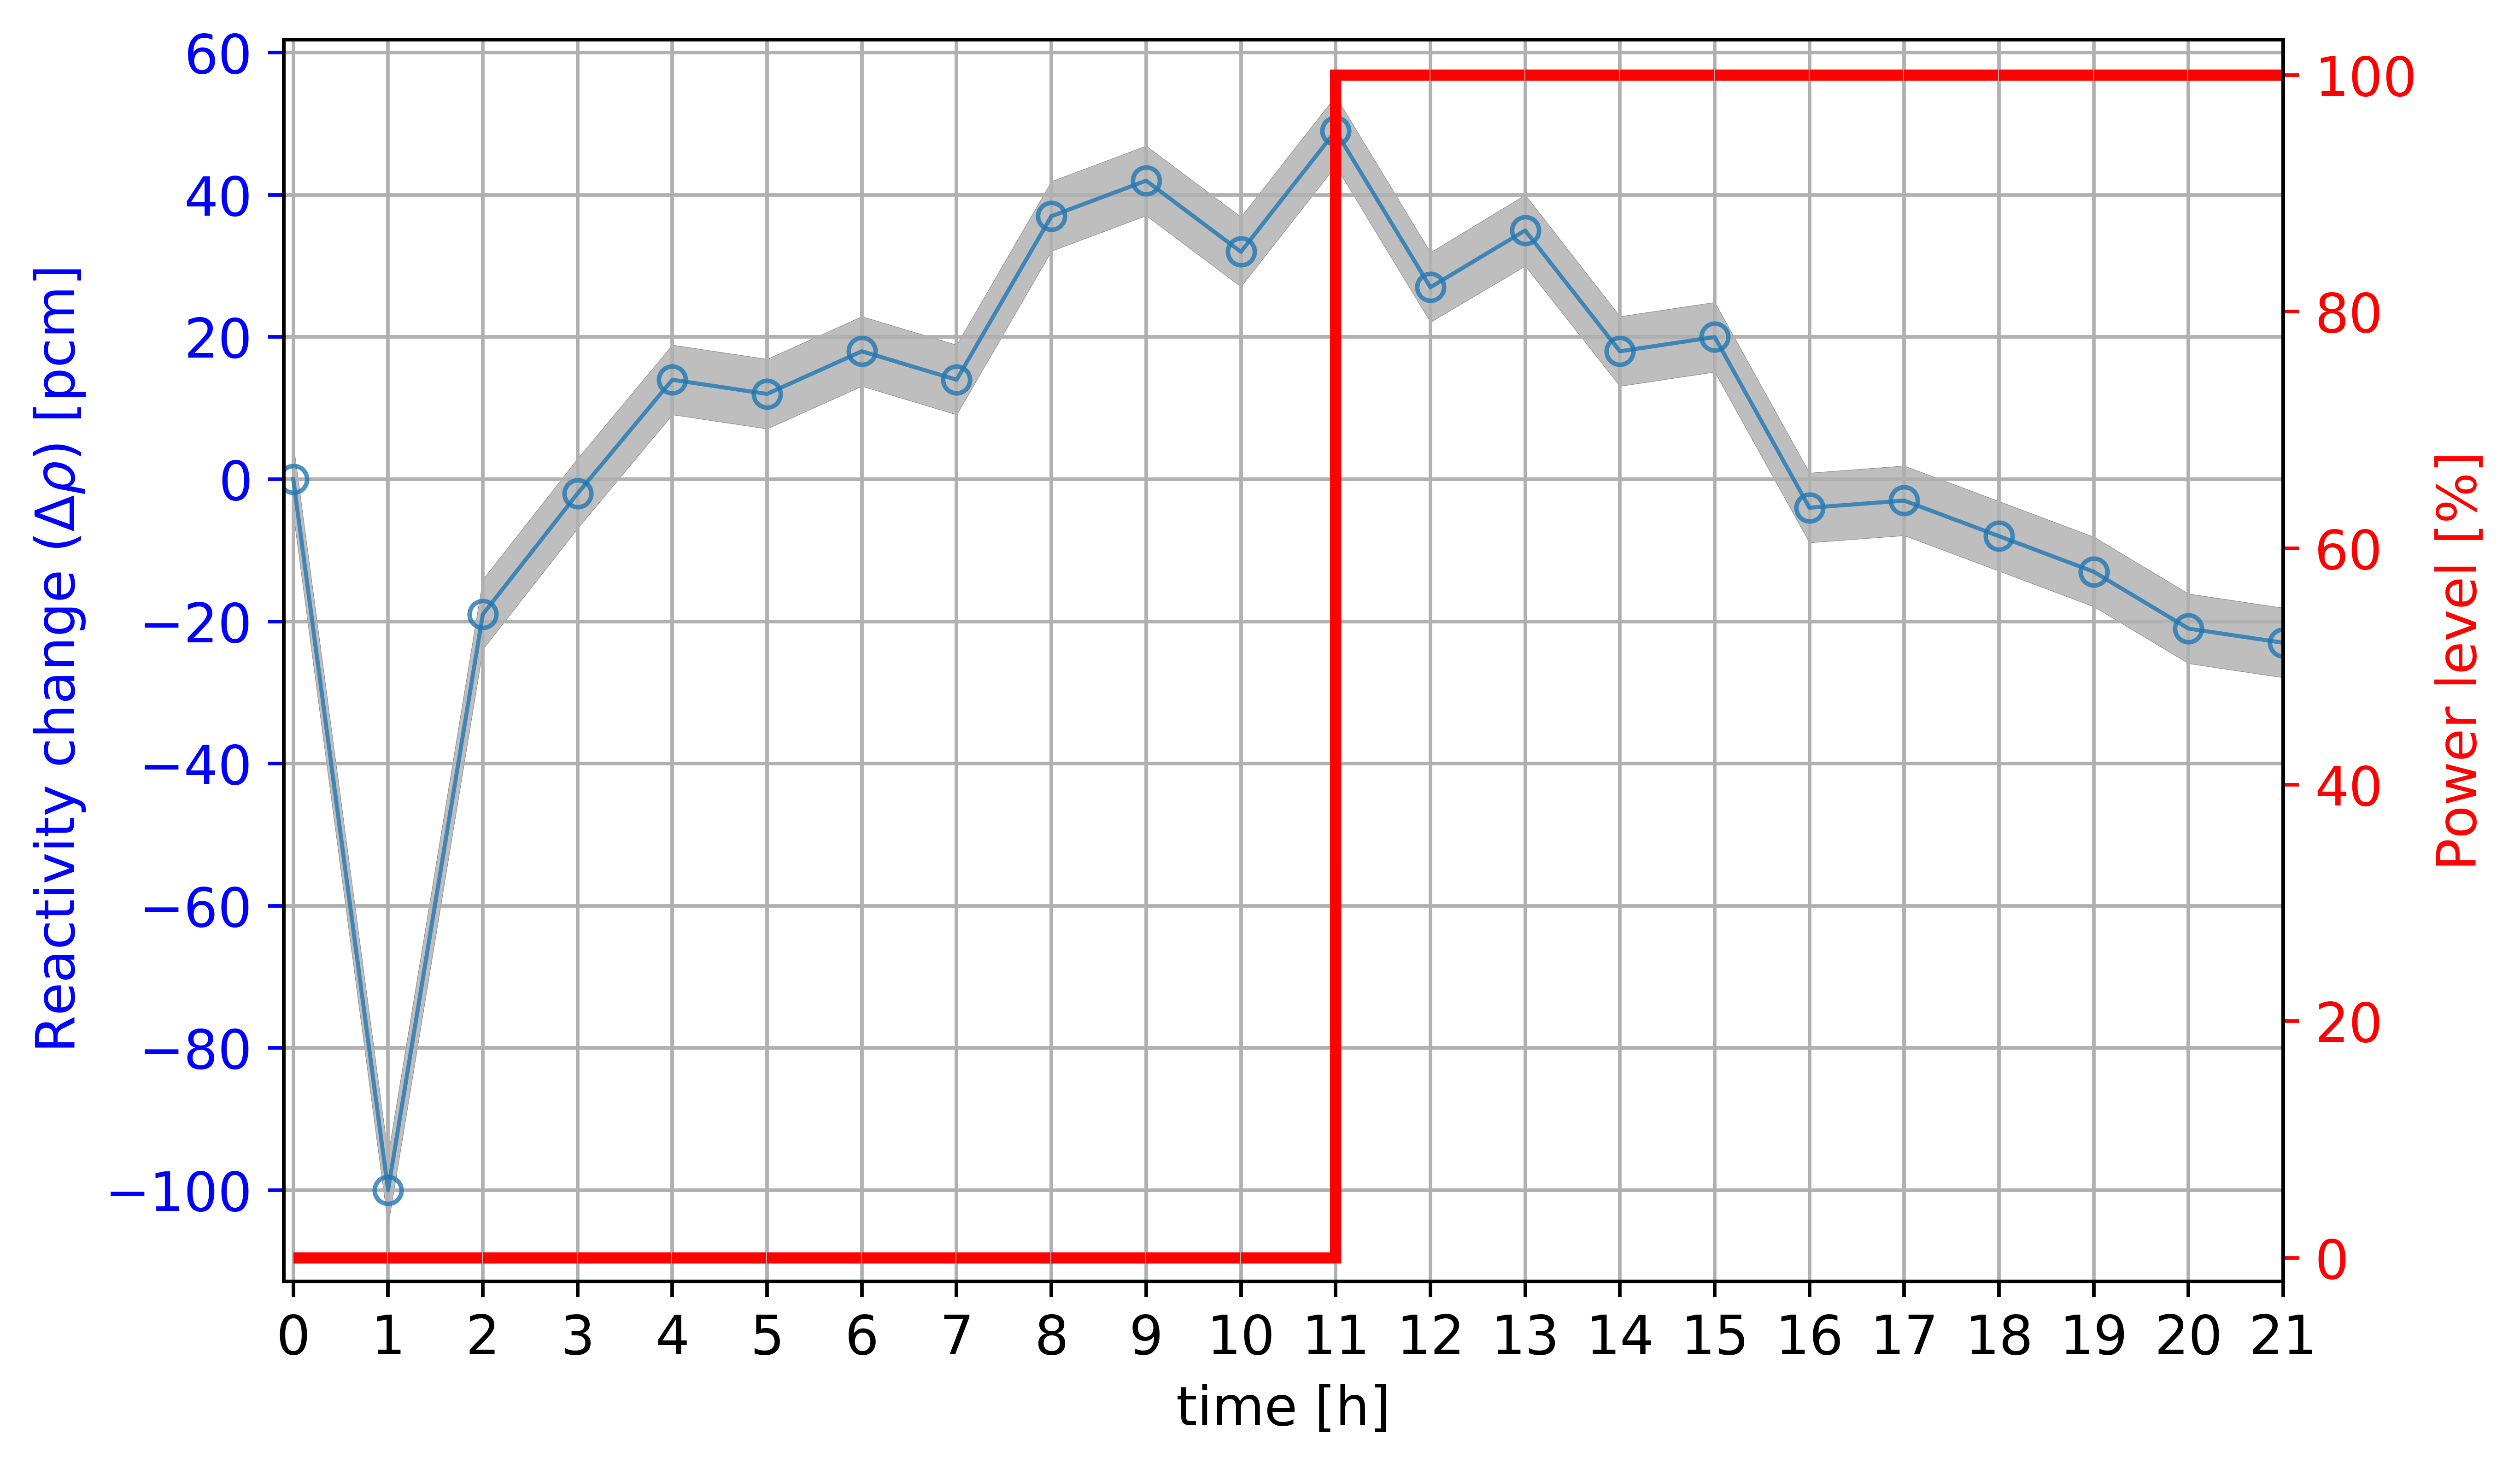
\includegraphics[width=0.97\textwidth]{ch5/rho_kl100_eol_eoc.png}
	\vspace{-5mm}
	\caption{Reactivity dynamics during an 11-hour shutdown for the 
		\gls{TAP} reactor, 10 days before the \gls{EOL} (all moderator rods 
		inserted), the gas removal system operates with efficiency 
		$\epsilon_{Xe}=0.915$. Uncertainty ($\sigma\pm5$ $pcm$) is 
		shaded.}
	\label{fig:lf-tap-rho-kl100-eol-eoc}
\end{figure}

Table~\ref{tab:lf-rho-change-eps-1} shows that the \gls{TAP} reactor with 
high gas removal efficiency experienced \emph{small effect of xenon poisoning} 
during the transient, and it also worsened toward the \gls{EOL}. Similar to 
the analysis with inactive gas removal 
system, maximum negative reactivity insertion due to xenon poisoning worsens 
toward the \gls{EOL} because $^{135}$Xe absorption cross section drops 
dramatically as energy grows. Notably, 
the maximum $^{135}$Xe concentration peak is significantly greater for an 
excellent gas removal efficiency ($\epsilon_{Xe}=0.915$) than for the 
no-removal case ($\epsilon_{Xe}=0$): +197\% and +4\%, respectively. Despite 
greater $^{135}$Xe concentration peak, negative change of reactivity after 
shutdown for the $\epsilon_{Xe}=0.915$ case is slightly deeper than for the 
$\epsilon_{Xe}=0$ case: -100 $pcm$ and -70 $pcm$, respectively. The reason for 
this is the neutron energy spectrum in the \gls{TAP} \gls{MSR}, which is 
harder than in conventional light-water thermal reactors. As we know, 
fast reactors are unaffected by xenon poisoning because the absorption cross 
section of $^{135}$Xe in the fast spectrum is insignificantly larger than 
absorption cross section of other fission products \cite{bell_nuclear_1970, 
svanstrom_load_2016-2}. The \gls{TAP} concept has intermediate spectrum which 
softens towards the \gls{EOL}. Finally, the effect of xenon 
poisoning in \gls{TAP} \gls{MSR} is almost negligible and can be easily 
compensated by control rod movement, while in well-studied \gls{PWR} it 
presents a challenge ($-1500$ $pcm$) \cite{rykhlevskii_impact_2019}.
%%%%%%%%%%%%%%%%%%%%%%%%%%%%%%%%%%%%%%%%%%%%%%%%%%%%%%%%%%%%%%%%%%%%%%%%%%%%%%%
\begin{table}[htp!]
	\centering
	\caption{Effect of $^{135}$Xe poisoning after shutdown for the 
		\gls{TAP} reactor operation with the high $^{135}$Xe removal 
		efficiency ($\epsilon_{Xe}=0.915$). Stochastic uncertainty 
		$\sigma_{\rho}=5$ $pcm$.}
	\begin{tabularx}{\textwidth}{p{0.06\textwidth} p{0.03\textwidth} R R R R 
			R}
		\hline
		Geo\-metry &	SVF [-] & Time after moderator configuration update 
		[d] & Operative excess reactivity ($\rho_0$) [$pcm$] & 
		$^{135}$I/$^{135}$Xe concentration ratio before shutdown
		[-] & Maximum relative $^{135}$Xe concentration 
		change [\%] & Maximum reactivity change after shutdown ($\Delta\rho$) 
		[$pcm$] \\ \hline
		1 & 0.903 & 9       & 3344 & 8.96  & +174 & -50  \\
    	1 & 0.903 & 171     & 1930 & 8.76  & +173 & -40  \\
		1 & 0.903 & 324     & 570  & 8.66  & +172 & -38  \\\hline
		8 & 0.766 & 3       & 3570 & 8.87  & +175 & -61  \\
		8 & 0.766 & 366     & 2150 & 8.90  & +174 & -40  \\
		8 & 0.766 & 762     & 762  & 8.93  & +175 & -33  \\\hline
		15& 0.536 & 9       & 3370 & 11.07 & +194 & -105  \\
		15& 0.536 & 90      & 2771 & 11.17 & +195 & -108  \\
		15& 0.536 & 303     & 1265 & 11.42 & +197 & -100  \\
		\hline
	\end{tabularx}
	\label{tab:lf-rho-change-eps-1}
\end{table}
%%%%%%%%%%%%%%%%%%%%%%%%%%%%%%%%%%%%%%%%%%%%%%%%%%%%%%%%%%%%%%%%%%%%%%%%%%%%%%%

Additionally, I analyzed the neutron spectrum of both reactors to understand 
the difference 
between $^{135}$I/$^{135}$Xe gain and loss for the \gls{TAP} \gls{MSR} and 
\gls{PWR}. Figure~\ref{fig:tap-pwr-spectrum} 
demonstrates the neutron flux energy distribution normalized by unit lethargy 
for both reactors. The \gls{TAP} reactor spectrum at the \gls{BOL} (SVF=0.903) 
is much harder than for the \gls{PWR} due to a lack of moderation in the 
\gls{TAP} core and its type (ZrH$_{1.66}$ instead of light water). The harder 
neutron spectrum leads to weaker $^{135}$Xe transmutation because the capture 
cross section declines rapidly with energy (see 
Figure~\ref{fig:tap-pwr-spectrum}, lower plot, solid red line, energy range 
from $10^{-7}$ to $10^{-4}$ MeV). As a result, the $^{135}$I/$^{135}$Xe number 
density ratio is 0.78 for the \gls{TAP} \gls{MSR} at the \gls{BOL}, which is 
significantly lower than that for the \gls{PWR} with fresh fuel (2.3). 
Thus, $^{135}$Xe gain from $^{135}$I decay cannot overcome $^{135}$Xe loss due 
to decay, and no xenon concentration peak is observed at the \gls{BOL} 
(Table~\ref{tab:lf-rho-change-eps-zero}, first three rows).
\begin{figure}[hbp!] % replace 't' with 'b' to 
	\centering
	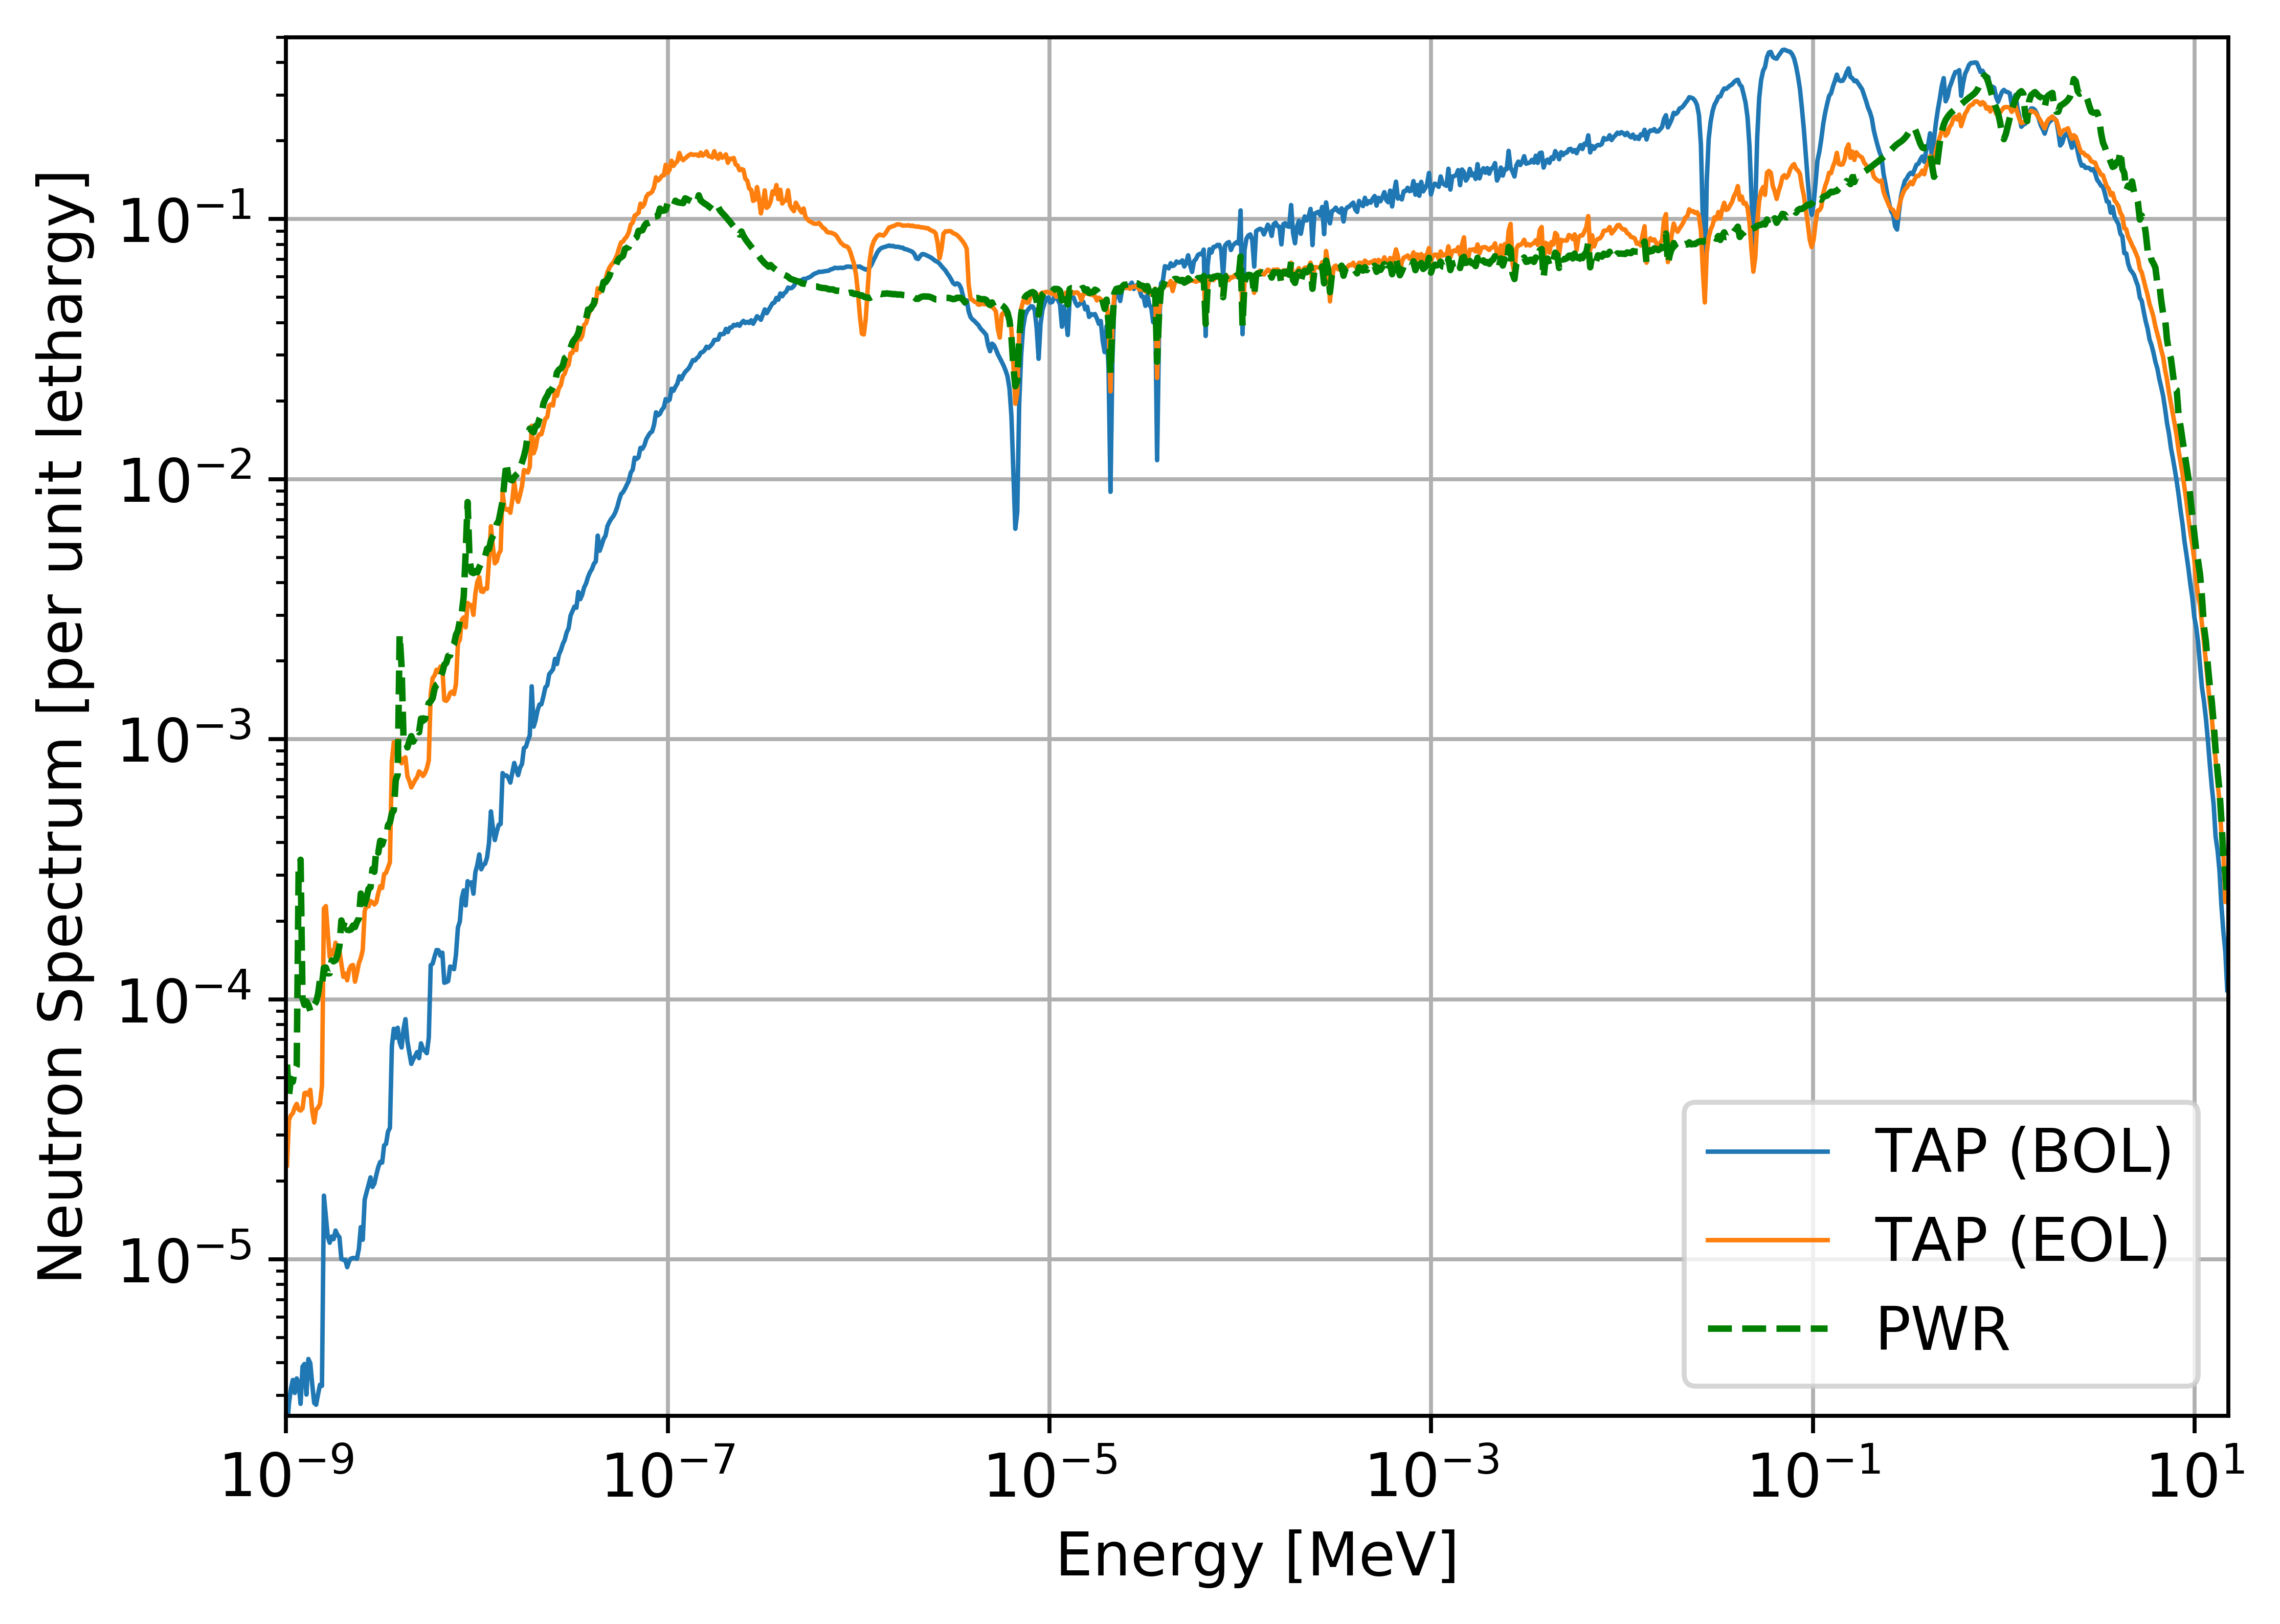
\includegraphics[width=\textwidth]{ch5/tap_vs_pwr_spectrum_2.png}\\
	\vspace{-19mm}
	\hspace{+0.05mm}
	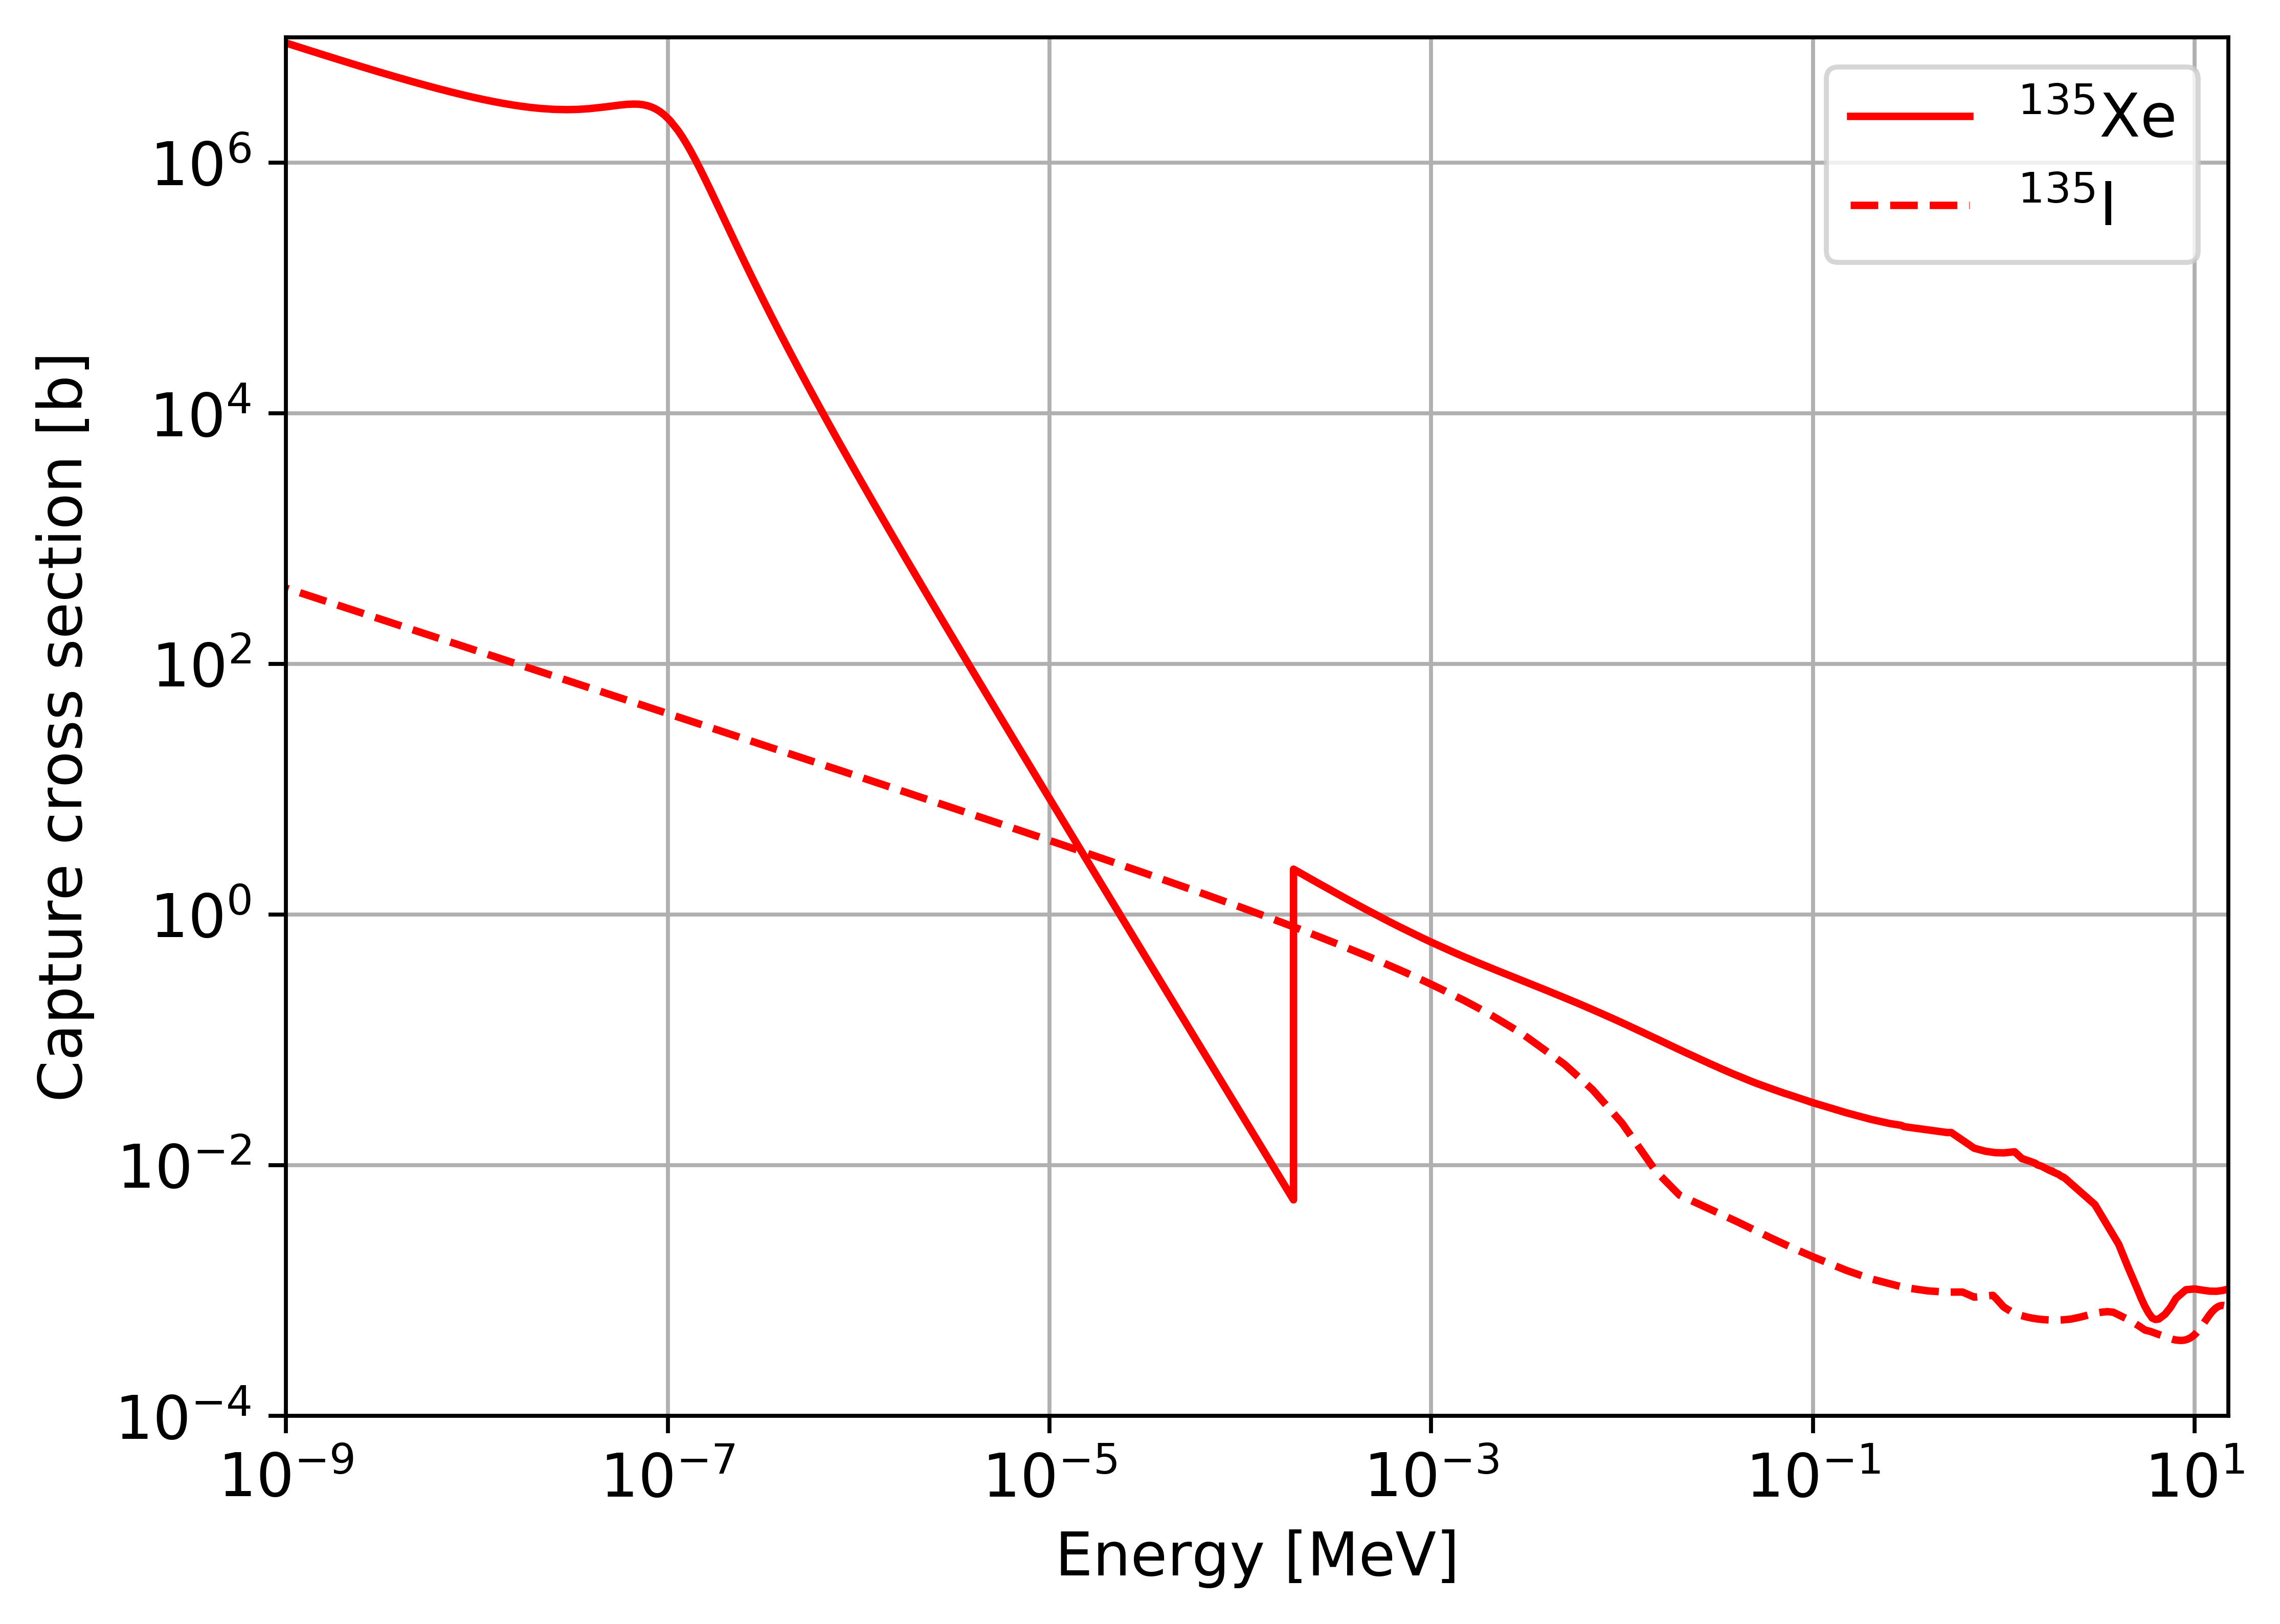
\includegraphics[width=\textwidth]{ch5/i_xe_xs.png}
	\vspace{-8mm}
	\caption{Neutron spectra normalized by lethargy for the \gls{PWR} and 
		\gls{TAP} (upper) and $^{135}$I, $^{135}$Xe caption cross 
		section (lower) \cite{rykhlevskii_impact_2019}.}
	\label{fig:tap-pwr-spectrum}
\end{figure}


The \gls{TAP} \gls{MSR} neutron spectrum thermalizes toward the \gls{EOL} due 
to additional moderator rod insertion. Figure~\ref{fig:tap-pwr-spectrum} 
shows that the \gls{TAP} core spectrum at the \gls{EOL} (after 23 years of 
operation, all moderator rods inserted into the core) is thermal and  similar 
to the \gls{PWR} spectrum. However, the $^{135}$I/$^{135}$Xe inventory ratio 
for the \gls{PWR} with fresh fuel is significantly greater than for the 
\gls{TAP} core at the \gls{EOL} despite similar spectra (2.3 and 1.0, 
respectively). The reason for that difference is the different fissile 
content. Results in Section~\ref{sec:long-term} shown that toward the 
\gls{EOL} fissile $^{235}$U is being substituted with fissile $^{239}$Pu and 
$^{241}$Pu. More specifically, instead of 6.8 t of $^{235}$U at startup, 
at the \gls{EOL}, the fuel salt contains 1.3 t of $^{235}$U, 1 t of 
$^{239}$Pu, and 0.5 t of $^{241}$Pu. That is, the fuel salt fissile inventory 
in the \gls{TAP} \gls{MSR} at the \gls{EOL} contains 46 wt\% of $^{235}$U, 36 
wt\% of $^{239}$Pu, and 18 wt\% of $^{241}$Pu.
%Once again, during the \gls{TAP} 
%\gls{MSR} operation a few major changes which impacted $^{135}$I/$^{135}$Xe 
%gain and loss are observed: (1) 
%neutron spectrum is shifted from fast to thermal 
%(Figure~\ref{fig:tap-pwr-spectrum});
%(2) fissile $^{235}$U is substituted with 
%fissile plutonium isotopes (e.g., $^{239}$Pu and $^{241}$Pu). 

Table~\ref{tab:fp-yield-thermal-fission} shows $^{135}$I and $^{135}$Xe yields 
from thermal fission for all fissile isotopes contained in the fuel 
salt. At the \gls{BOL}, $^{135}$I and $^{135}$Xe in the \gls{TAP} 
reactor and \gls{PWR} are produced from $^{235}$U fission. The $^{135}$I 
isotope production rate  per thermal fission stays approximately the same 
during 23 years of operation because $^{135}$I yield is very close for all 
considered fissile isotopes. However, the rate of $^{135}$Xe production 
directly from fission for 
fissile plutonium isotopes is significantly greater than for the $^{235}$U 
(e.g., $\approx5$ times greater for $^{239}$Pu and $\approx8$ times greater 
for $^{241}$Pu). Thus, a greater $^{135}$Xe production rate toward \gls{EOL} 
with approximately the same $^{135}$I production rate leads to a smaller 
$^{135}$I/$^{135}$Xe concentration ratio. Overall, $^{135}$I/$^{135}$Xe 
number density ratio increasing from 0.78 to 1.0 during 25 years of the 
\gls{TAP} \gls{MSR} operation, which leads to a more massive $^{135}$Xe 
concentration peak after shutdown and worsens xenon poisoning effect.
%%%%%%%%%%%%%%%%%%%%%%%%%%%%%%%%%%%%%%%%
\begin{table}[htp!]
	\centering
	\caption{Fission product yields (isotopes per fission) from thermal 
	fission 
	\cite{nichols_handbook_2008}.}
	\begin{tabularx}{0.6\textwidth}{p{0.12\textwidth} R R R}
		\hline
		\textbf{Isotope}  & \textbf{$^{235}$U} &		
		\textbf{$^{239}$Pu} & \textbf{$^{241}$Pu} \\ \hline
		$^{135}$I  & 0.0639 & 0.0633 & 0.0684 \\
		$^{135}$Xe & 0.0022 & 0.0103 & 0.0017 \\
		\hline
	\end{tabularx}
	\label{tab:fp-yield-thermal-fission}
\end{table}
%%%%%%%%%%%%%%%%%%%%%%%%%%%%%%%%%%%%%%%%%%%%%%%%%%%%%%%%%%%%%%%%%%%%%%%%%%%%%%%
%%%%%%%%%%%%%%%%%%%%%%%%%%%%%%%%%%%%%%%%
%\begin{table}[htp!]
%	\centering
%	\caption{Fission product yields (atoms per fission) from fast fission 
%	\cite{nichols_handbook_2008}.}
%	\begin{tabularx}{0.6\textwidth}{p{0.12\textwidth} R R R }
%		\hline
%		\textbf{Isotope}  & \textbf{$^{235}$U} & 
%		\textbf{$^{239}$Pu} & \textbf{$^{241}$Pu} \\ \hline
%		$^{135}$I  & 0.0601 & 0.0624 & 0.0696 \\
%		$^{135}$Xe & 0.0031 & 0.0126 & 0.0030 \\
%		\hline
%	\end{tabularx}
%	\label{tab:fp-yield-fast-fission}
%\end{table}
%%%%%%%%%%%%%%%%%%%%%%%%%%%%%%%%%%%%%%%%%%%%%%%%%%%%%%%%%%%%%%%%%%%%%%%%%%%%%%%

In conclusion, I observed a negligible xenon poisoning in the \gls{TAP} 
reactor during the anticipated transient because it has a relatively hard 
neutron energy spectrum even at the most thermal core configuration (all 
moderator rods are inserted into the core). The harder spectrum gives 
a small $^{135}$I/$^{135}$Xe concentration ratio which leads to a low
$^{135}$Xe concentration peak after the shutdown. Notably, the fission gas 
removal with high efficiency did not significantly change the xenon poisoning 
effect because the $^{135}$Xe absorption cross section fell dramatically as 
neutron energy grows. Overall, the \gls{TAP} reactor can effectively 
load-follow even without fission gas removal. 

\section{Safety and operational parameters evolution during load following} 
\label{ch5:saf_param}
To analyze the impact of the load-following transient on the \gls{TAP} concept 
safety, I calculated safety and operational parameters at various moments 
during postulated earlier worst-case power change transient (0\% power level 
for 11 hours, instantaneous power boost to 100\%, and then 10 hours on 100\% 
power level) using methodology from Section~\ref{sec:safety-param}. The 
combination of fuel and moderator temperature feedback coefficients must 
remain negative, and the reactivity worth of control rods must be sufficient 
to shut down the reactor throughout the transient. Ideally, the reactor is 
more controllable if major safety and operational parameters remain stable and 
unaffected by the substantial power level change.

\subsection{Temperature coefficient of reactivity}
Figure~\ref{fig:lf-tap-tc-evo} shows the temperature feedback coefficient 
evolution for the \gls{TAP} reactor during the power change transient. The 
Fuel Temperature Coefficient ($\alpha_{T,F}$) became less negative during the 
first hour of the transient due to a slight spectrum hardening because the  
$^{135}$Xe concentration peak changes the Doppler effect in the fuel salt. 
After turning the power back on, all three temperature coefficients of 
reactivity remains stable because the fuel salt composition remain almost 
unchanged. Overall, the isothermal temperature coefficient, $\alpha_{T,ISO}$ 
remains negative and strong throughout the postulated transient and 
fluctuates slightly within stochastic error range 
$\sigma_{\alpha_{T,ISO}}\pm0.043$ $pcm/K$. 
\begin{figure}[htp!] % replace 't' with 'b' to 
	\centering
	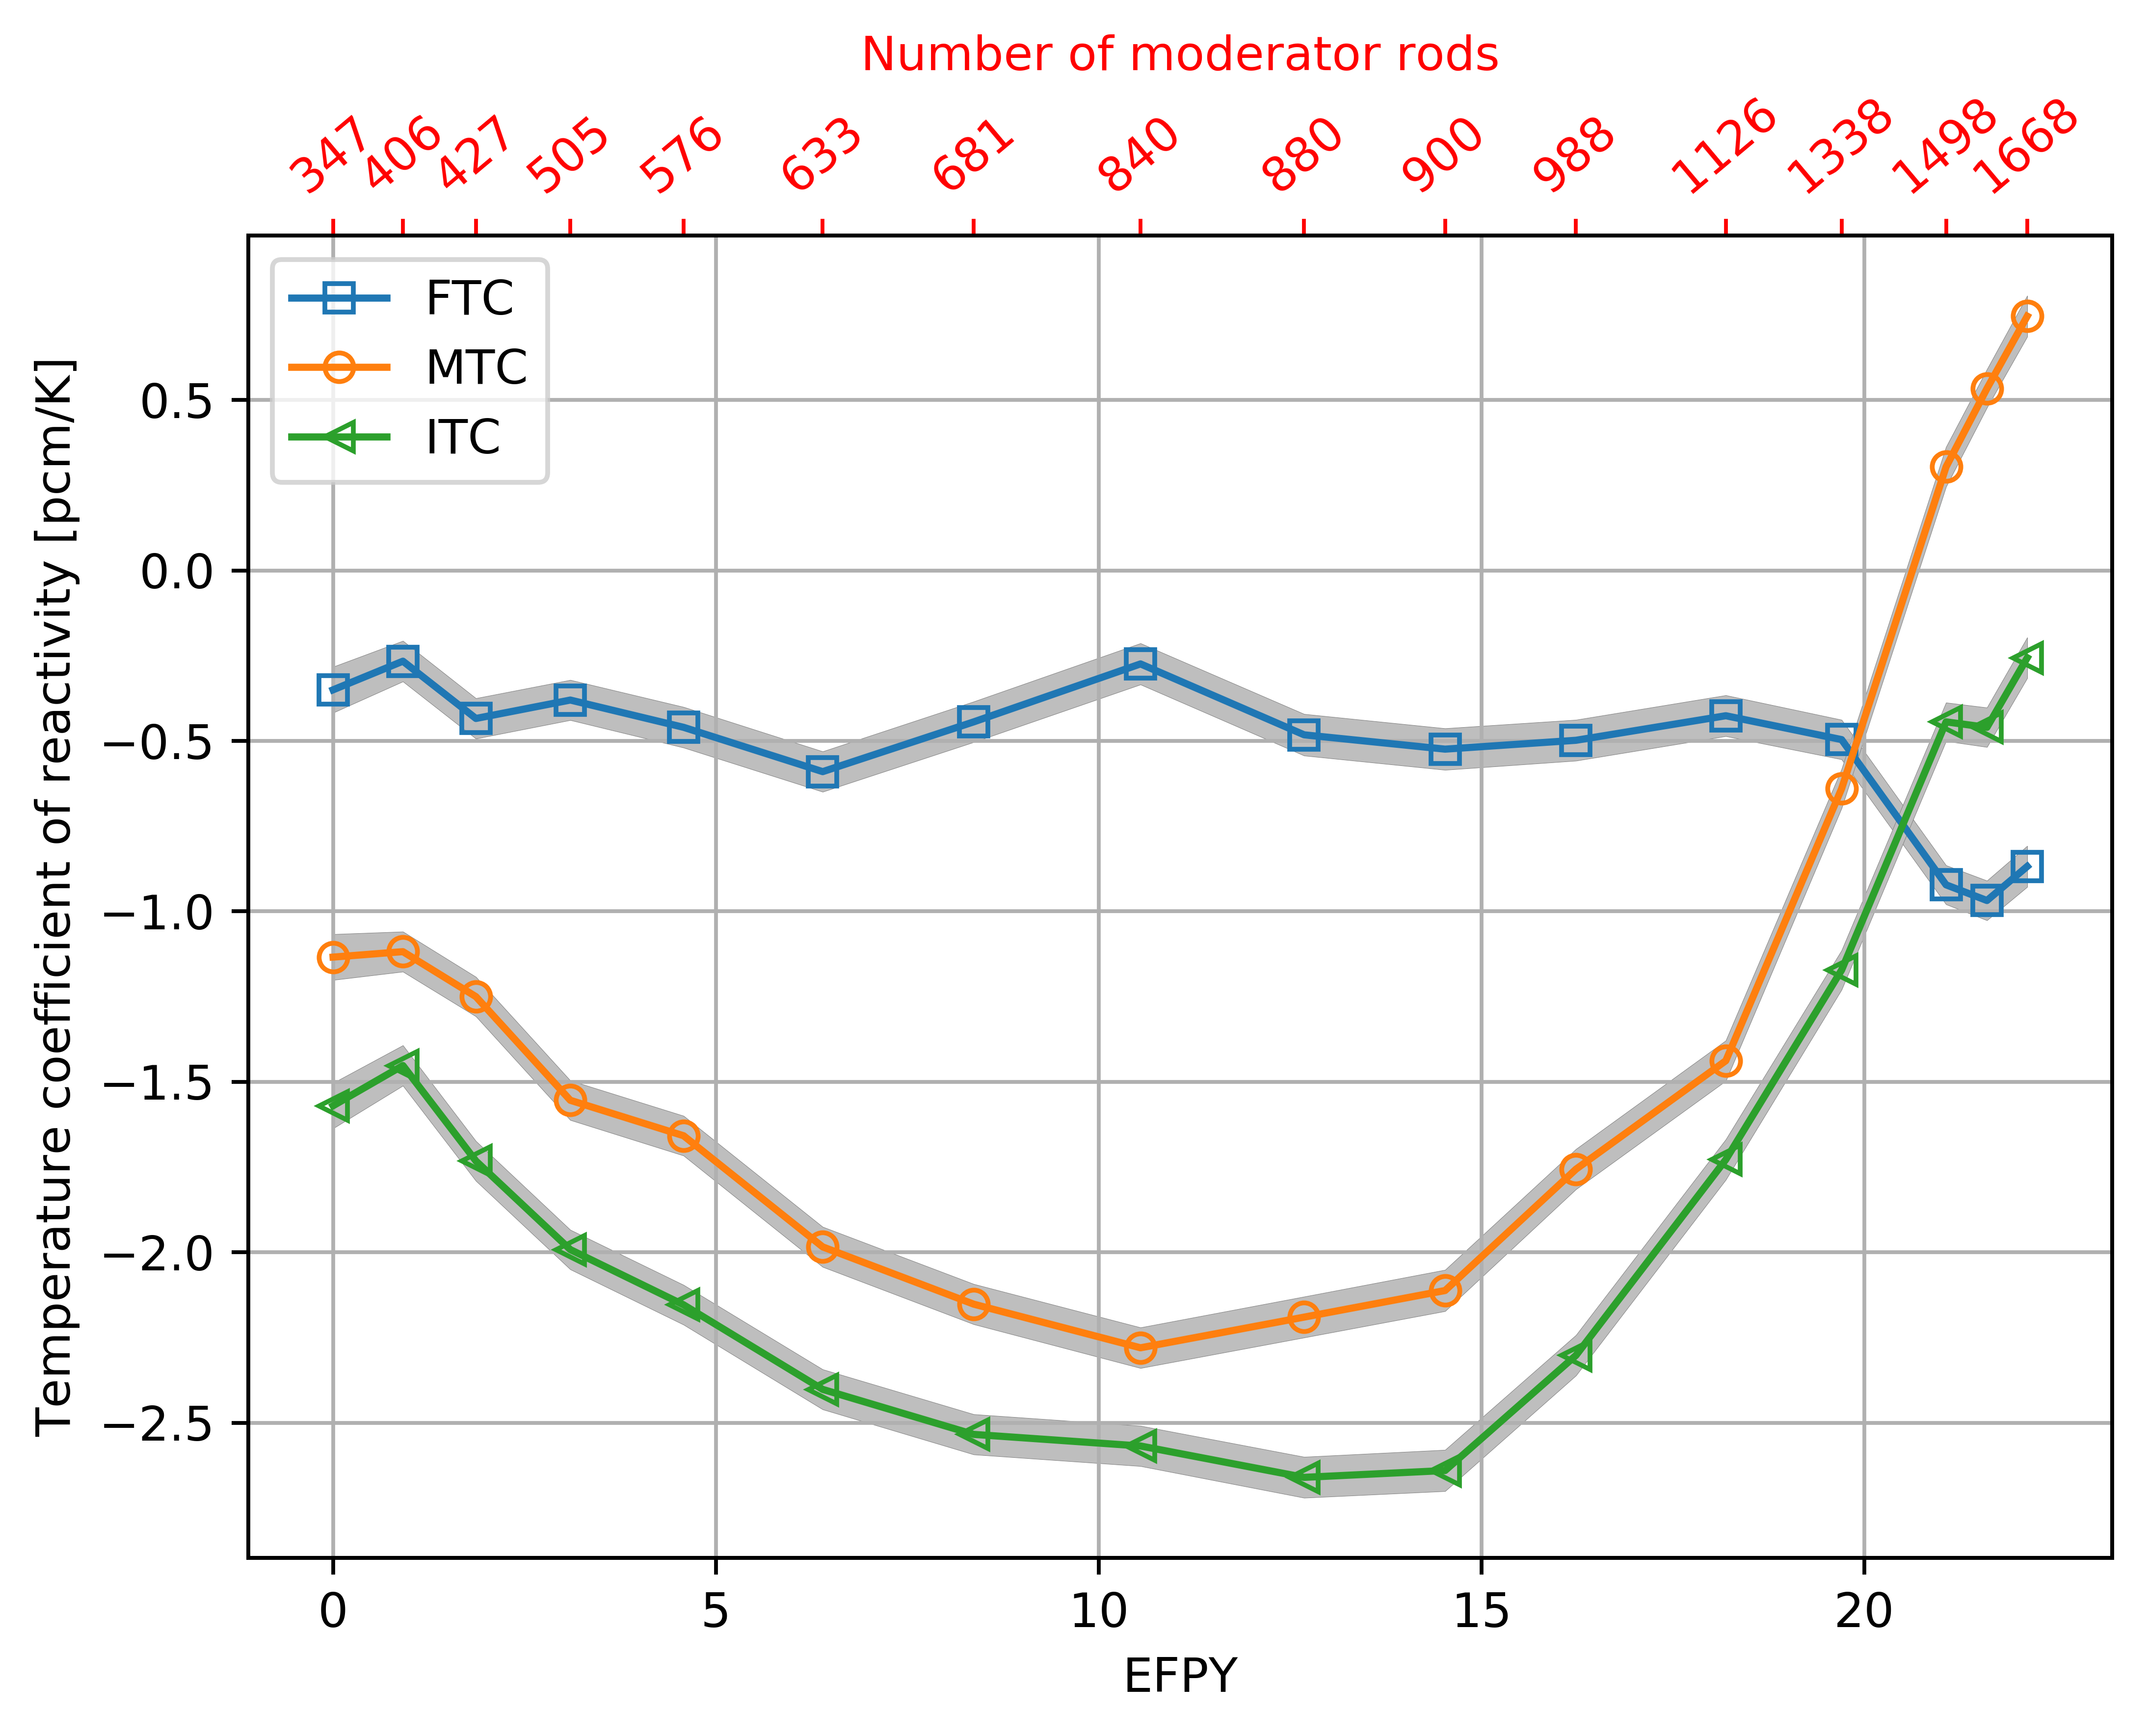
\includegraphics[width=\textwidth]{ch5/saf_par/tc_evo.png}
	\caption{Temperature feedback coefficients during the postulated 
		transient for the \gls{TAP} reactor, 10 days before the \gls{EOL} (all 
		moderator rods inserted), the gas removal system operates with 
		efficiency $\epsilon_{Xe}=0.915$. The uncertainty, $\pm\sigma$, is 
		shaded.}
		\label{fig:lf-tap-tc-evo}
\end{figure}

\subsection{Void coefficient of reactivity}
Figure~\ref{fig:lf-tap-void-evo} demonstrates the void coefficient of 
reactivity evolution during the postulated transient. 
The $\alpha_V$ remains almost constant throughout the postulated transient. 
All observed changes in the void coefficient of reactivity are due to the
stochastic nature of the Monte Carlo method ($\sigma_{\alpha_V}\pm4$ $pcm/$\%).
\begin{figure}[htp!] % replace 't' with 'b' to 
	\centering
	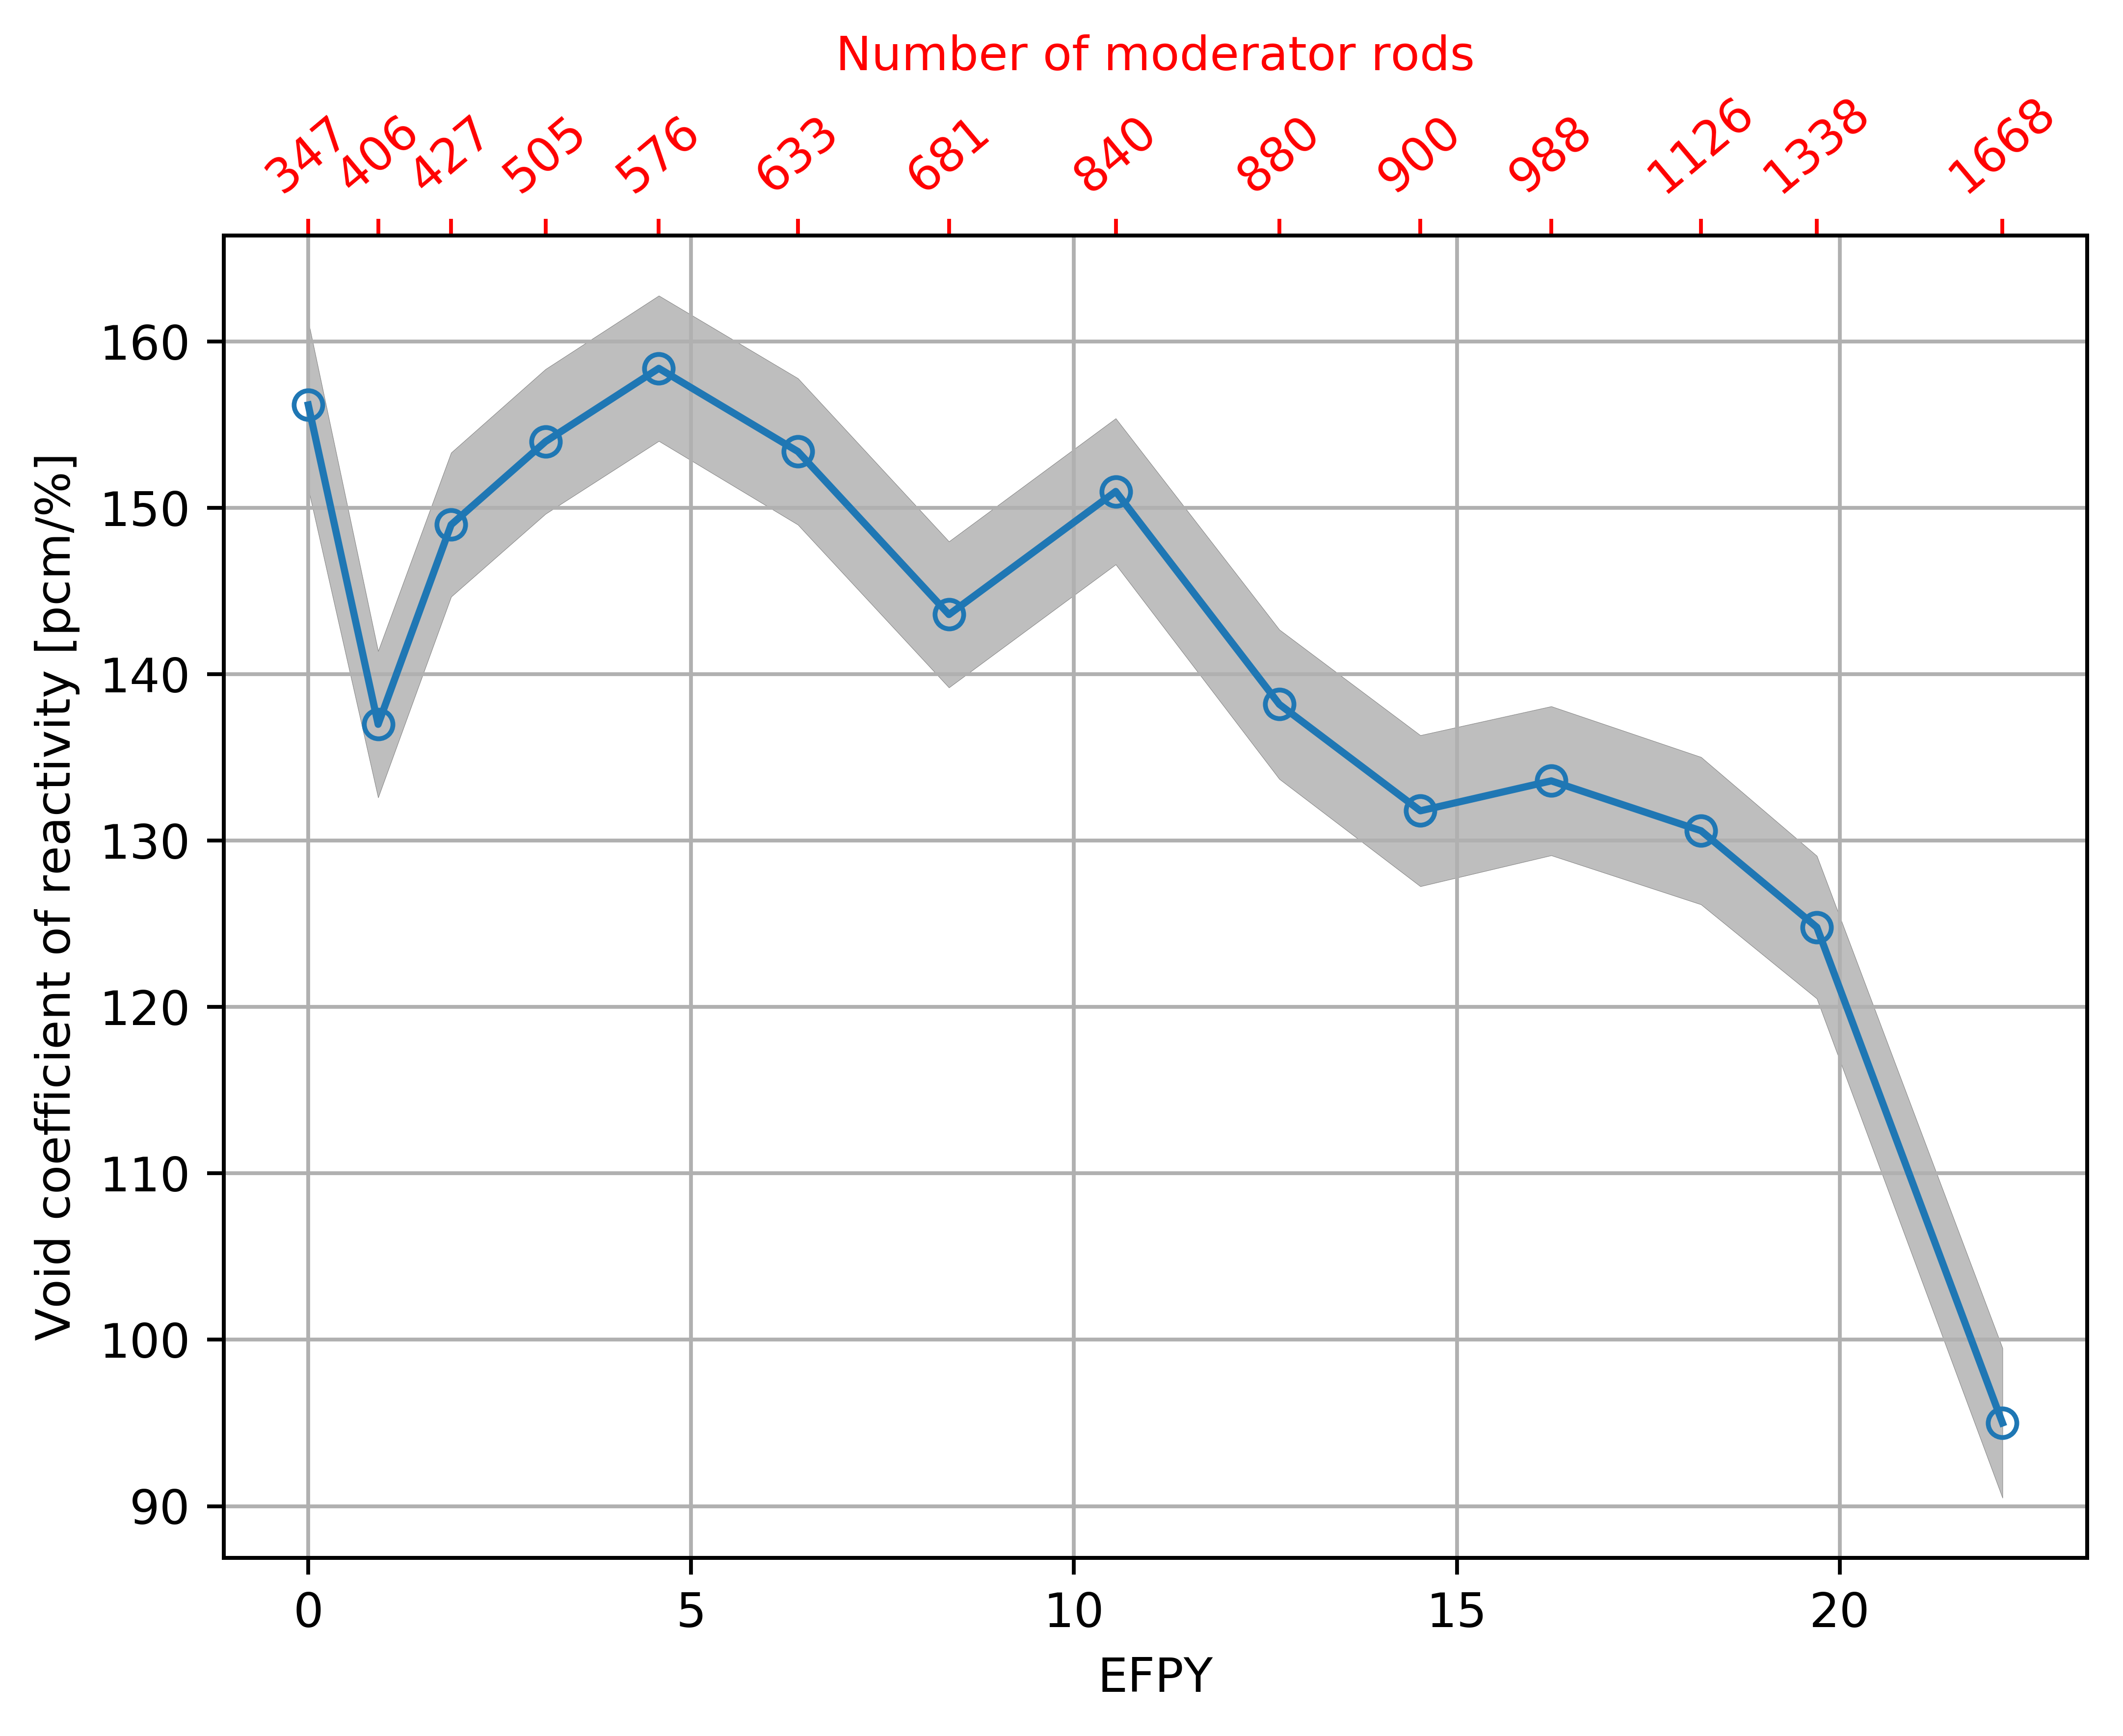
\includegraphics[width=\textwidth]{ch5/saf_par/void_evo.png}
	\caption{Void coefficient of reactivity as a function of time during 
	postulated transient for the \gls{TAP} reactor, 10 days before the 
	\gls{EOL} (all moderator rods inserted), the gas removal system operates 
	with efficiency $\epsilon_{Xe}=0.915$.}
	\label{fig:lf-tap-void-evo}
\end{figure}

\subsection{Reactivity control rod worth}
Figure~\ref{fig:lf-tap-crw-evo} demonstrates the control rod worth evolution 
during the power change transient. The control rod worth remains almost 
constant and sufficient to shut down the reactor throughout the postulated 
transient. During the first three hours of the transient, the control rod 
worth decreases from $1998.9\pm8.9$ $pcm$ to $1988.3\pm8.9$ $pcm$ due to a 
slight spectrum hardening caused by $^{135}$Xe concentration raise. Overall, 
the control rod worth changes are insignificant and lie within the 
stochastic error range ($\sigma_{CRW}\pm8.9$ $pcm$).
\begin{figure}[htp!] % replace 't' with 'b' to 
	\centering
	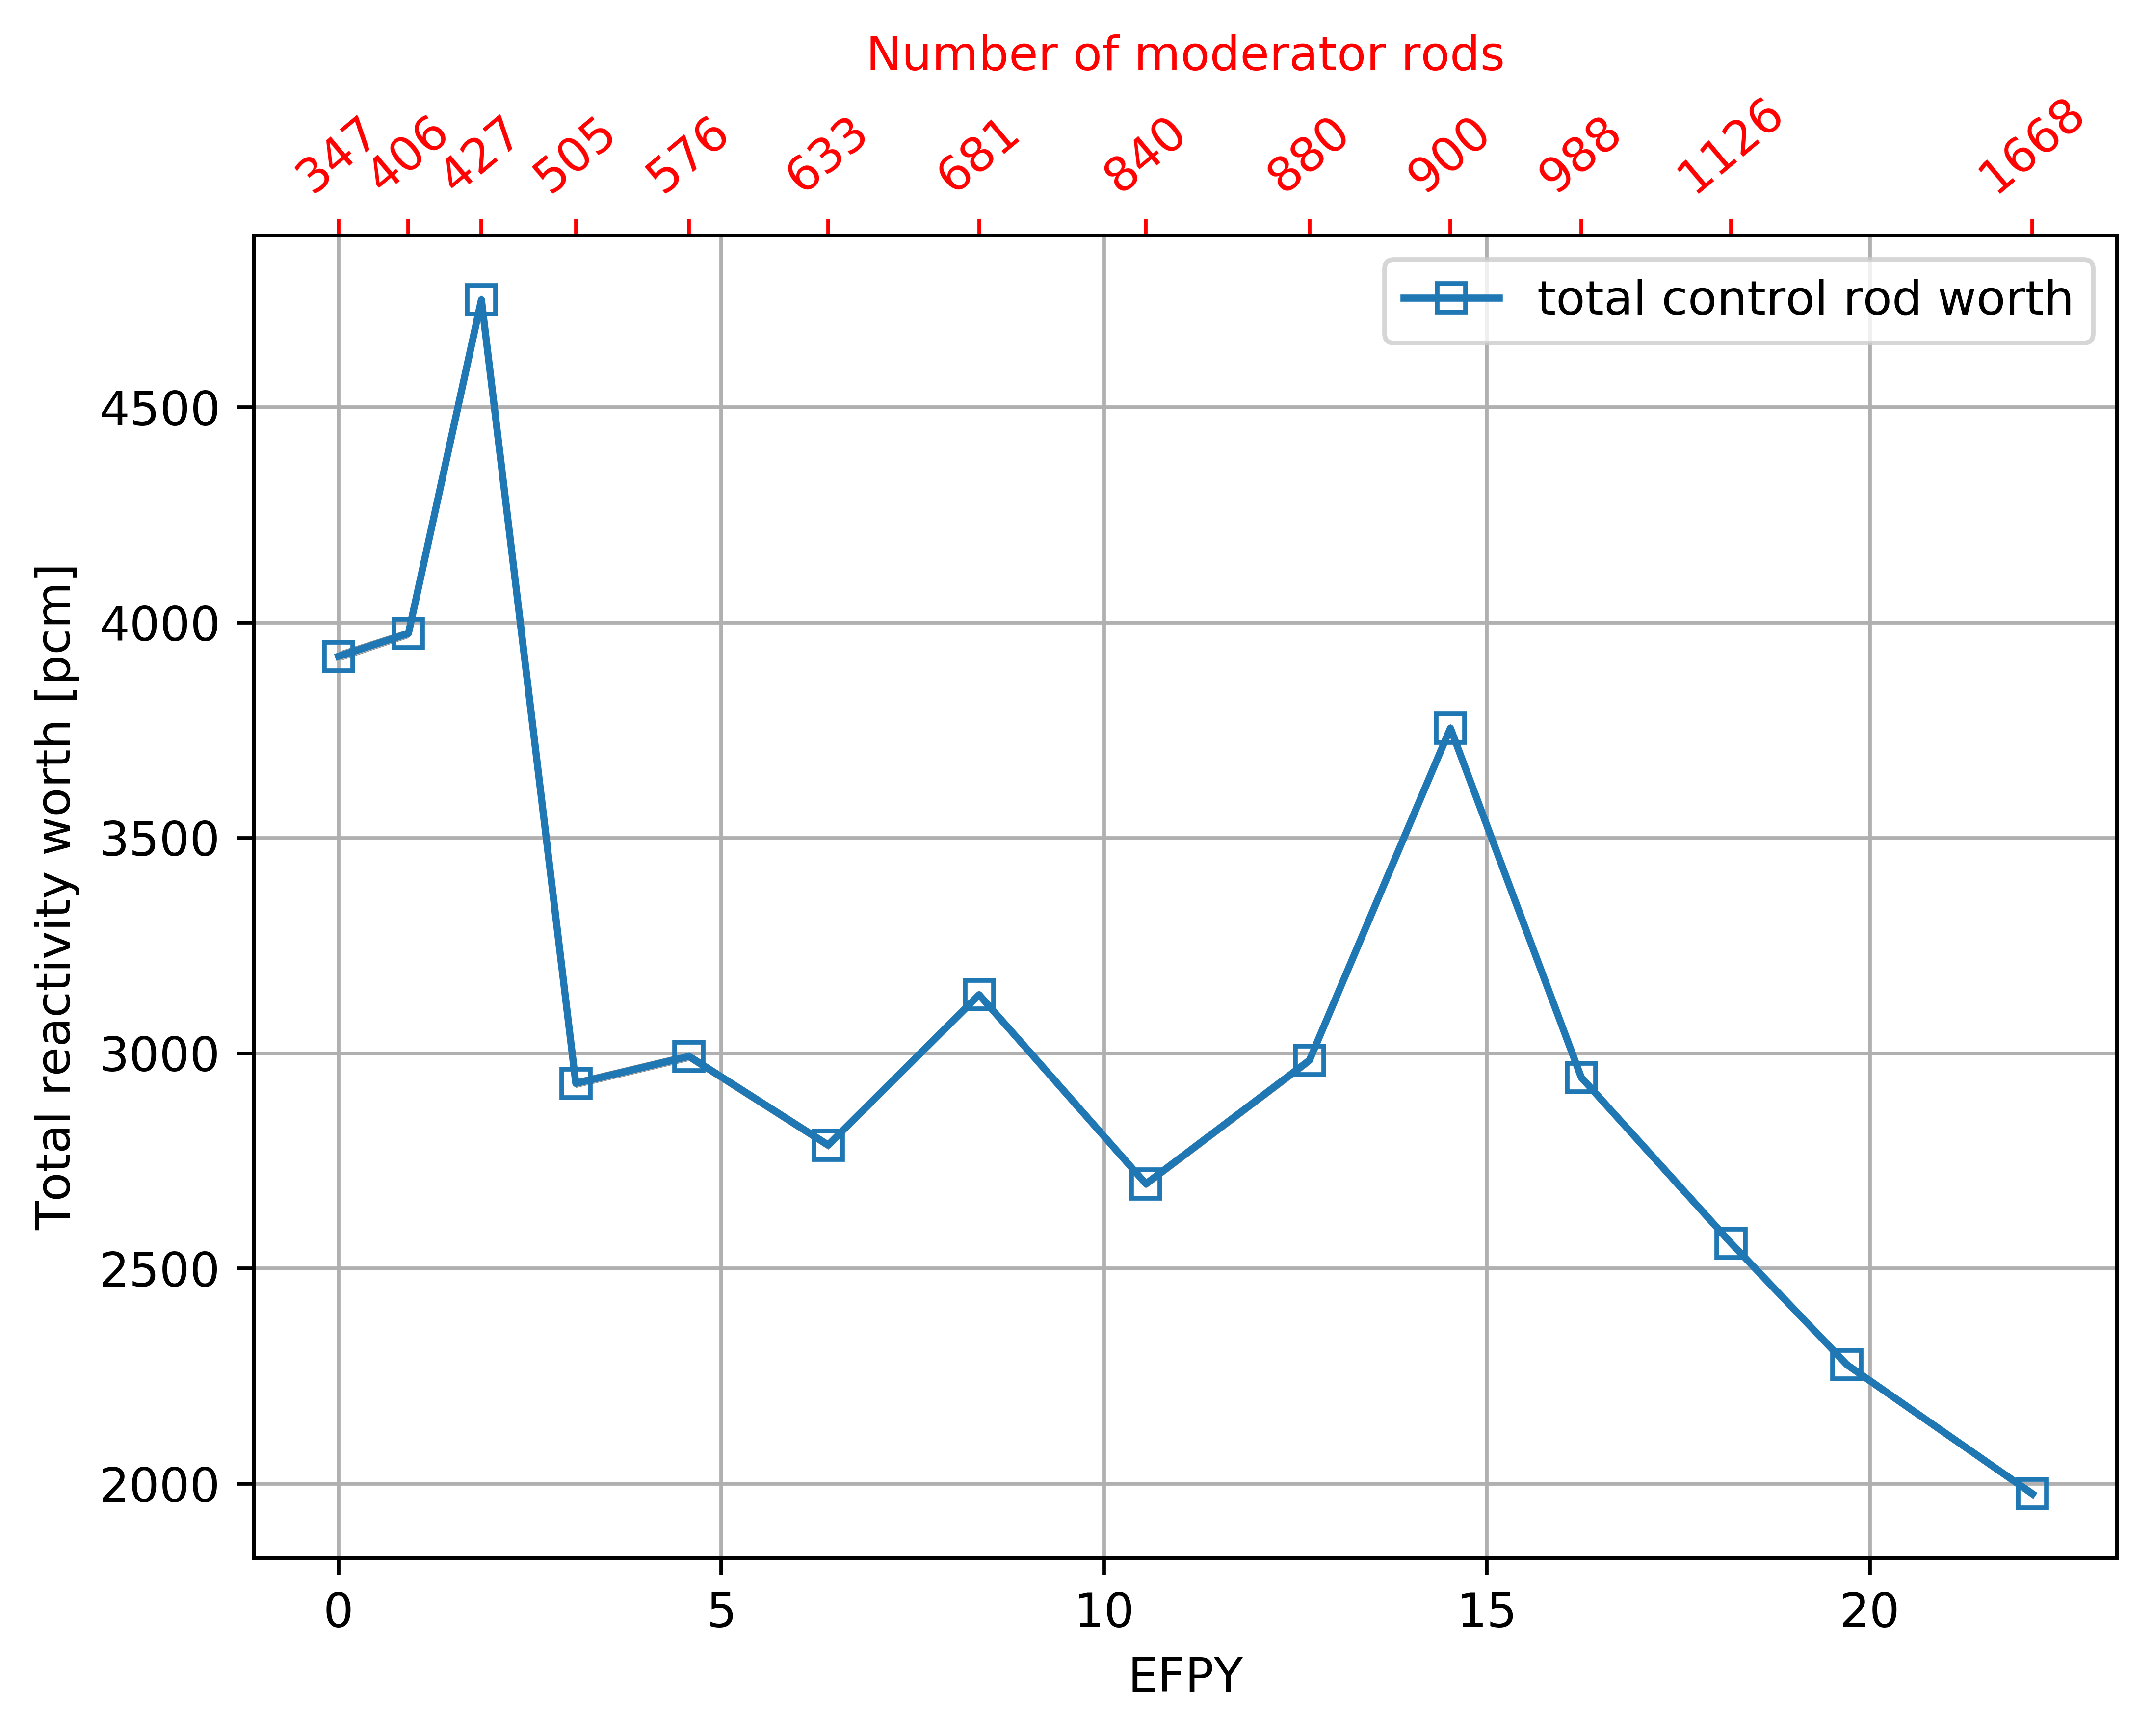
\includegraphics[width=\textwidth]{ch5/saf_par/crw_evo.png}
	\caption{Total control rod worth as a function of time during postulated 
	transient for the \gls{TAP} reactor, 10 days before the \gls{EOL} (all 
	moderator rods inserted), the gas removal system operates with efficiency 
	$\epsilon_{Xe}=0.915$.}
	\label{fig:lf-tap-crw-evo}
\end{figure}



\section{Concluding remarks}
This chapter demonstrated the short-term depletion simulations for the 
\gls{TAP} reactor with the core power level variation in the range of [0, 
100\%] using SaltProc v1.0 and Serpent. I considered two different noble gas 
removal scenarios: (1) no gas removal (e.g., $\epsilon_{Xe}=0$), 
and (2) fully operational gas removal system (e.g., $\epsilon_{Xe}=0.915$). 
The results in the literature reported that negative xenon poisoning effect 
for conventional \glspl{LWR} reaches its extremum $\Delta\rho\approx-1500$ 
$pcm$ in approximately 11 hours after shutdown. Such a vast reactivity drop 
complicates the \glspl{LWR} load-following.

For the case with no gas removal ($\epsilon_{Xe}=0$), $^{135}$Xe 
concentration peaks about 45 and 165 min after the shutdown at the 
\gls{BOL} and \gls{EOL}, respectively. The xenon concentration peaks 
sooner for the harder core configuration (e.g., at the \gls{BOL}, SVF=0.9) 
because $^{135}$Xe absorption cross section drops dramatically as neutron 
energy grows above 0.1 eV, thus, $^{135}$Xe burn out faster in a harder 
spectrum. Thus, the harder spectrum leads to a smaller $^{135}$I/$^{135}$Xe 
concentration ratio and, consequently, lower xenon concentration peak after 
shutdown. Without gas removal (e.g., $^{135}$Xe loss after 
shutdown due to decay only) xenon concentration at the \gls{BOL} remains 
almost constant ($\Delta N_{^{135}Xe}=+0.33$\%), and no effect of xenon 
poisoning was observed ($\Delta\rho=-10\pm7$ $pcm$). However, at the 
\gls{EOL}, when all moderator rods are in and the neutron spectrum is more 
thermal, I observed a more significant effect of poisoning: $^{135}$Xe 
concentration increased by 4\% with corresponding negative reactivity 
insertion of $-70$ $pcm$. 

For the case with very effective noble gas removal ($\epsilon_{Xe}=0.915$), 
the time when $^{135}$Xe concentration peaks cannot be predicted analytically, 
because, after shutdown, the gas removal system removes a major 
fraction of xenon gas at the end of each depletion step. Moreover, the 
$^{135}$I/$^{135}$Xe ratio is significantly greater (e.g., between 8.66 and 
11.42) than for the non-removal ($\epsilon_{Xe}=0$) case. Thus, $^{135}$I 
decay leads to 
a substantial increase in $^{135}$Xe concentration right after shutdown (up to 
+200\% at the \gls{EOL}), and corresponding reactivity drop ($-108\pm5$ $pcm$ 
at the \gls{EOL}). However, after the first hour, reactivity increases quickly 
because the gas removal system extracts most of the xenon every 1 hour (the 
selected SaltProc v1.0 depletion time step). The true effect of xenon 
poisoning for the \gls{TAP} reactor with active gas removal is expected to be 
even less severe because the real system would remove noble gases 
continuously, not discretely as simulated by SaltProc (e.g., xenon would be 
removed with $\epsilon_{Xe}=0.915$ every moment, not once per hour). Overall, 
more realistic results for load-following transients can be obtained with 
better time resolution. Though the ideal depletion time step should be closer 
to full loop time (20 seconds), such fidelity would require an enormous 
computation burden.

Finally, this chapter demonstrated that the \gls{TAP} reactor maintains 
required safety margins during postulated transients. The temperature feedback 
coefficients, void coefficient of reactivity, and control rod worth all remain 
within stochastic uncertainty throughout the transient. Small elevation in 
total temperature coefficient and void coefficient of reactivity during the 
first hour after shutdown is due to the $^{135}$Xe concentration raise and 
corresponding short-term neutron spectrum hardening. In conclusion, the 
\gls{TAP} \gls{MSR}, even without gas removal, is capable of the safe restart 
after reducing power from 100\% to 0\% even when $^{135}$Xe concentration 
peaks. 
While this work has confirmed neutronics feasibility of resilience against the 
iodine pit, separate thermomechanical structural analysis is needed to confirm 
that structural materials could withstand such dramatic core power 
fluctuations.
%The comprehensive material study must be done to prove that structural 
%materials could withstand such dramatic core power fluctuations.





